% Options for packages loaded elsewhere
\PassOptionsToPackage{unicode}{hyperref}
\PassOptionsToPackage{hyphens}{url}
%
\documentclass[
  english,
  man,floatsintext]{apa6}
\usepackage{amsmath,amssymb}
\usepackage{lmodern}
\usepackage{ifxetex,ifluatex}
\ifnum 0\ifxetex 1\fi\ifluatex 1\fi=0 % if pdftex
  \usepackage[T1]{fontenc}
  \usepackage[utf8]{inputenc}
  \usepackage{textcomp} % provide euro and other symbols
\else % if luatex or xetex
  \usepackage{unicode-math}
  \defaultfontfeatures{Scale=MatchLowercase}
  \defaultfontfeatures[\rmfamily]{Ligatures=TeX,Scale=1}
\fi
% Use upquote if available, for straight quotes in verbatim environments
\IfFileExists{upquote.sty}{\usepackage{upquote}}{}
\IfFileExists{microtype.sty}{% use microtype if available
  \usepackage[]{microtype}
  \UseMicrotypeSet[protrusion]{basicmath} % disable protrusion for tt fonts
}{}
\makeatletter
\@ifundefined{KOMAClassName}{% if non-KOMA class
  \IfFileExists{parskip.sty}{%
    \usepackage{parskip}
  }{% else
    \setlength{\parindent}{0pt}
    \setlength{\parskip}{6pt plus 2pt minus 1pt}}
}{% if KOMA class
  \KOMAoptions{parskip=half}}
\makeatother
\usepackage{xcolor}
\IfFileExists{xurl.sty}{\usepackage{xurl}}{} % add URL line breaks if available
\IfFileExists{bookmark.sty}{\usepackage{bookmark}}{\usepackage{hyperref}}
\hypersetup{
  pdftitle={Peekbank: An open, large-scale repository for developmental eye-tracking data of children's word recognition},
  pdfauthor={Martin Zettersten1, Daniel Yurovsky2, Tian Linger Xu3, Sarp Uner4, Angeline Sin Mei Tsui5, Rose M. Schneider6, Annissa N. Saleh7, Stephan Meylan8,9, Virginia Marchman5, Jessica Mankewitz5, Kyle MacDonald10, Bria Long5, Molly Lewis2, George Kachergis5, Kunal Handa11, Benjamin deMayo1, Alexandra Carstensen6, Mika Braginsky9, Veronica Boyce5, Naiti S. Bhatt12, Claire Bergey13, \& Michael C. Frank5},
  pdflang={en-EN},
  pdfkeywords={word recognition; eye-tracking; vocabulary development; looking-while-listening; visual world paradigm; lexical processing},
  hidelinks,
  pdfcreator={LaTeX via pandoc}}
\urlstyle{same} % disable monospaced font for URLs
\usepackage{color}
\usepackage{fancyvrb}
\newcommand{\VerbBar}{|}
\newcommand{\VERB}{\Verb[commandchars=\\\{\}]}
\DefineVerbatimEnvironment{Highlighting}{Verbatim}{commandchars=\\\{\}}
% Add ',fontsize=\small' for more characters per line
\usepackage{framed}
\definecolor{shadecolor}{RGB}{248,248,248}
\newenvironment{Shaded}{\begin{snugshade}}{\end{snugshade}}
\newcommand{\AlertTok}[1]{\textcolor[rgb]{0.94,0.16,0.16}{#1}}
\newcommand{\AnnotationTok}[1]{\textcolor[rgb]{0.56,0.35,0.01}{\textbf{\textit{#1}}}}
\newcommand{\AttributeTok}[1]{\textcolor[rgb]{0.77,0.63,0.00}{#1}}
\newcommand{\BaseNTok}[1]{\textcolor[rgb]{0.00,0.00,0.81}{#1}}
\newcommand{\BuiltInTok}[1]{#1}
\newcommand{\CharTok}[1]{\textcolor[rgb]{0.31,0.60,0.02}{#1}}
\newcommand{\CommentTok}[1]{\textcolor[rgb]{0.56,0.35,0.01}{\textit{#1}}}
\newcommand{\CommentVarTok}[1]{\textcolor[rgb]{0.56,0.35,0.01}{\textbf{\textit{#1}}}}
\newcommand{\ConstantTok}[1]{\textcolor[rgb]{0.00,0.00,0.00}{#1}}
\newcommand{\ControlFlowTok}[1]{\textcolor[rgb]{0.13,0.29,0.53}{\textbf{#1}}}
\newcommand{\DataTypeTok}[1]{\textcolor[rgb]{0.13,0.29,0.53}{#1}}
\newcommand{\DecValTok}[1]{\textcolor[rgb]{0.00,0.00,0.81}{#1}}
\newcommand{\DocumentationTok}[1]{\textcolor[rgb]{0.56,0.35,0.01}{\textbf{\textit{#1}}}}
\newcommand{\ErrorTok}[1]{\textcolor[rgb]{0.64,0.00,0.00}{\textbf{#1}}}
\newcommand{\ExtensionTok}[1]{#1}
\newcommand{\FloatTok}[1]{\textcolor[rgb]{0.00,0.00,0.81}{#1}}
\newcommand{\FunctionTok}[1]{\textcolor[rgb]{0.00,0.00,0.00}{#1}}
\newcommand{\ImportTok}[1]{#1}
\newcommand{\InformationTok}[1]{\textcolor[rgb]{0.56,0.35,0.01}{\textbf{\textit{#1}}}}
\newcommand{\KeywordTok}[1]{\textcolor[rgb]{0.13,0.29,0.53}{\textbf{#1}}}
\newcommand{\NormalTok}[1]{#1}
\newcommand{\OperatorTok}[1]{\textcolor[rgb]{0.81,0.36,0.00}{\textbf{#1}}}
\newcommand{\OtherTok}[1]{\textcolor[rgb]{0.56,0.35,0.01}{#1}}
\newcommand{\PreprocessorTok}[1]{\textcolor[rgb]{0.56,0.35,0.01}{\textit{#1}}}
\newcommand{\RegionMarkerTok}[1]{#1}
\newcommand{\SpecialCharTok}[1]{\textcolor[rgb]{0.00,0.00,0.00}{#1}}
\newcommand{\SpecialStringTok}[1]{\textcolor[rgb]{0.31,0.60,0.02}{#1}}
\newcommand{\StringTok}[1]{\textcolor[rgb]{0.31,0.60,0.02}{#1}}
\newcommand{\VariableTok}[1]{\textcolor[rgb]{0.00,0.00,0.00}{#1}}
\newcommand{\VerbatimStringTok}[1]{\textcolor[rgb]{0.31,0.60,0.02}{#1}}
\newcommand{\WarningTok}[1]{\textcolor[rgb]{0.56,0.35,0.01}{\textbf{\textit{#1}}}}
\usepackage{graphicx}
\makeatletter
\def\maxwidth{\ifdim\Gin@nat@width>\linewidth\linewidth\else\Gin@nat@width\fi}
\def\maxheight{\ifdim\Gin@nat@height>\textheight\textheight\else\Gin@nat@height\fi}
\makeatother
% Scale images if necessary, so that they will not overflow the page
% margins by default, and it is still possible to overwrite the defaults
% using explicit options in \includegraphics[width, height, ...]{}
\setkeys{Gin}{width=\maxwidth,height=\maxheight,keepaspectratio}
% Set default figure placement to htbp
\makeatletter
\def\fps@figure{htbp}
\makeatother
\setlength{\emergencystretch}{3em} % prevent overfull lines
\providecommand{\tightlist}{%
  \setlength{\itemsep}{0pt}\setlength{\parskip}{0pt}}
\setcounter{secnumdepth}{-\maxdimen} % remove section numbering
% Make \paragraph and \subparagraph free-standing
\ifx\paragraph\undefined\else
  \let\oldparagraph\paragraph
  \renewcommand{\paragraph}[1]{\oldparagraph{#1}\mbox{}}
\fi
\ifx\subparagraph\undefined\else
  \let\oldsubparagraph\subparagraph
  \renewcommand{\subparagraph}[1]{\oldsubparagraph{#1}\mbox{}}
\fi
% Manuscript styling
\usepackage{upgreek}
\captionsetup{font=singlespacing,justification=justified}

% Table formatting
\usepackage{longtable}
\usepackage{lscape}
% \usepackage[counterclockwise]{rotating}   % Landscape page setup for large tables
\usepackage{multirow}		% Table styling
\usepackage{tabularx}		% Control Column width
\usepackage[flushleft]{threeparttable}	% Allows for three part tables with a specified notes section
\usepackage{threeparttablex}            % Lets threeparttable work with longtable

% Create new environments so endfloat can handle them
% \newenvironment{ltable}
%   {\begin{landscape}\centering\begin{threeparttable}}
%   {\end{threeparttable}\end{landscape}}
\newenvironment{lltable}{\begin{landscape}\centering\begin{ThreePartTable}}{\end{ThreePartTable}\end{landscape}}

% Enables adjusting longtable caption width to table width
% Solution found at http://golatex.de/longtable-mit-caption-so-breit-wie-die-tabelle-t15767.html
\makeatletter
\newcommand\LastLTentrywidth{1em}
\newlength\longtablewidth
\setlength{\longtablewidth}{1in}
\newcommand{\getlongtablewidth}{\begingroup \ifcsname LT@\roman{LT@tables}\endcsname \global\longtablewidth=0pt \renewcommand{\LT@entry}[2]{\global\advance\longtablewidth by ##2\relax\gdef\LastLTentrywidth{##2}}\@nameuse{LT@\roman{LT@tables}} \fi \endgroup}

% \setlength{\parindent}{0.5in}
% \setlength{\parskip}{0pt plus 0pt minus 0pt}

% \usepackage{etoolbox}
\makeatletter
\patchcmd{\HyOrg@maketitle}
  {\section{\normalfont\normalsize\abstractname}}
  {\section*{\normalfont\normalsize\abstractname}}
  {}{\typeout{Failed to patch abstract.}}
\patchcmd{\HyOrg@maketitle}
  {\section{\protect\normalfont{\@title}}}
  {\section*{\protect\normalfont{\@title}}}
  {}{\typeout{Failed to patch title.}}
\makeatother
\shorttitle{Peekbank repository for eye-tracking data}
\keywords{word recognition; eye-tracking; vocabulary development; looking-while-listening; visual world paradigm; lexical processing\newline\indent Word count: 7351}
\usepackage{lineno}

\linenumbers
\usepackage{csquotes}
\usepackage{setspace}
\ifxetex
  % Load polyglossia as late as possible: uses bidi with RTL langages (e.g. Hebrew, Arabic)
  \usepackage{polyglossia}
  \setmainlanguage[]{english}
\else
  \usepackage[main=english]{babel}
% get rid of language-specific shorthands (see #6817):
\let\LanguageShortHands\languageshorthands
\def\languageshorthands#1{}
\fi
\ifluatex
  \usepackage{selnolig}  % disable illegal ligatures
\fi
\newlength{\cslhangindent}
\setlength{\cslhangindent}{1.5em}
\newlength{\csllabelwidth}
\setlength{\csllabelwidth}{3em}
\newenvironment{CSLReferences}[2] % #1 hanging-ident, #2 entry spacing
 {% don't indent paragraphs
  \setlength{\parindent}{0pt}
  % turn on hanging indent if param 1 is 1
  \ifodd #1 \everypar{\setlength{\hangindent}{\cslhangindent}}\ignorespaces\fi
  % set entry spacing
  \ifnum #2 > 0
  \setlength{\parskip}{#2\baselineskip}
  \fi
 }%
 {}
\usepackage{calc}
\newcommand{\CSLBlock}[1]{#1\hfill\break}
\newcommand{\CSLLeftMargin}[1]{\parbox[t]{\csllabelwidth}{#1}}
\newcommand{\CSLRightInline}[1]{\parbox[t]{\linewidth - \csllabelwidth}{#1}\break}
\newcommand{\CSLIndent}[1]{\hspace{\cslhangindent}#1}

\title{Peekbank: An open, large-scale repository for developmental eye-tracking data of children's word recognition}
\author{Martin Zettersten\textsuperscript{1}, Daniel Yurovsky\textsuperscript{2}, Tian Linger Xu\textsuperscript{3}, Sarp Uner\textsuperscript{4}, Angeline Sin Mei Tsui\textsuperscript{5}, Rose M. Schneider\textsuperscript{6}, Annissa N. Saleh\textsuperscript{7}, Stephan Meylan\textsuperscript{8,9}, Virginia Marchman\textsuperscript{5}, Jessica Mankewitz\textsuperscript{5}, Kyle MacDonald\textsuperscript{10}, Bria Long\textsuperscript{5}, Molly Lewis\textsuperscript{2}, George Kachergis\textsuperscript{5}, Kunal Handa\textsuperscript{11}, Benjamin deMayo\textsuperscript{1}, Alexandra Carstensen\textsuperscript{6}, Mika Braginsky\textsuperscript{9}, Veronica Boyce\textsuperscript{5}, Naiti S. Bhatt\textsuperscript{12}, Claire Bergey\textsuperscript{13}, \& Michael C. Frank\textsuperscript{5}}
\date{}


\authornote{

\textbf{Acknowledgements.} We would like to thank the labs and researchers that have made their data publicly available in the database. For further information about contributions, see \url{https://langcog.github.io/peekbank-website/docs/contributors/}.

\textbf{Open Practices Statement.} All code for reproducing the paper is available at \url{https://github.com/langcog/peekbank-paper}. Raw and standardized datasets are available on the Peekbank OSF repository (\url{https://osf.io/pr6wu/}) and can be accessed using the peekbankr R package (\url{https://github.com/langcog/peekbankr}).

\textbf{CRediT author statement.} Outside of the position of the first and the last author, authorship position was determined by sorting authors' last names in reverse alphabetical order. An overview of authorship contributions following the CRediT taxonomy can be viewed here: \url{https://docs.google.com/spreadsheets/d/e/2PACX-1vRD-LJD_dTAQaAynyBlwXvGpfAVzP-3Pi6JTDoG15m3PYZe0c44Y12U2a_hwdmhIstpjyigG2o3na4y/pubhtml}.

Correspondence concerning this article should be addressed to Martin Zettersten, Department of Psychology, Princeton University, 218 Peretsman Scully Hall, Princeton, NJ 08540. E-mail: \href{mailto:martincz@princeton.edu}{\nolinkurl{martincz@princeton.edu}}

}

\affiliation{\vspace{0.5cm}\textsuperscript{1} Department of Psychology, Princeton University\\\textsuperscript{2} Department of Psychology, Carnegie Mellon University\\\textsuperscript{3} Department of Psychological and Brain Sciences, Indiana University\\\textsuperscript{4} Data Science Institute, Vanderbilt University\\\textsuperscript{5} Department of Psychology, Stanford University\\\textsuperscript{6} Department of Psychology, University of California, San Diego\\\textsuperscript{7} Department of Psychology, The University of Texas at Austin\\\textsuperscript{8} Department of Psychology and Neuroscience, Duke University\\\textsuperscript{9} Department of Brain and Cognitive Sciences, Massachusetts Institute of Technology\\\textsuperscript{10} Core Technology, McD Tech Labs\\\textsuperscript{11} Brown University\\\textsuperscript{12} Department of Psychology, New York University\\\textsuperscript{13} Department of Psychology, University of Chicago}

\abstract{
The ability to rapidly recognize words and link them to referents is central to children's early language development.
This ability, often called word recognition in the developmental literature, is typically studied in the looking-while-listening paradigm, which measures infants' fixation on a target object (vs.~a distractor) after hearing a target label.
We present a large-scale, open database of infant and toddler eye-tracking data from looking-while-listening tasks.
The goal of this effort is to address theoretical and methodological challenges in measuring vocabulary development.
We first present how we created the database, its features and structure, and associated tools for processing and accessing infant eye-tracking datasets.
Using these tools, we then work through two illustrative examples to show how researchers can use Peekbank to interrogate theoretical and methodological questions about children's developing word recognition ability.
}



\begin{document}
\maketitle

Across their first years of life, children learn words at an accelerating pace (Frank, Braginsky, Yurovsky, \& Marchman, 2021).
While many children will only produce their first word at around one year of age, most children show signs of understanding many common nouns (e.g., \emph{mommy}) and phrases (e.g., \emph{Let's go bye-bye!}) much earlier in development (Bergelson \& Swingley, 2012, 2013; Tincoff \& Jusczyk, 1999).
Although early word understanding is a critical element of first language learning, the processes involved are less directly apparent in children's behaviors and are less accessible to observation than developments in speech production (Fernald, Zangl, Portillo, \& Marchman, 2008; Hirsh-Pasek, Cauley, Golinkoff, \& Gordon, 1987).
To understand a spoken word, children must process the incoming auditory signal and link that signal to relevant meanings -- a process often referred to as word recognition.
One of the primary means of measuring word recognition in young infants is using eye-tracking techniques that gauge where children look in response to linguistic stimuli (Fernald, Zangl, Portillo, \& Marchman, 2008).
The logic of these methods is that if, upon hearing a word, a child preferentially looks at a target stimulus rather than a distractor, the child is able to recognize the word and activate its meaning during real-time language processing.
Measuring early word recognition offers insight into children's early word representations: children's speed of response (i.e., moving their eyes; turning their heads) to the unfolding speech signal can reveal children's level of comprehension (Bergelson, 2020; Fernald, Pinto, Swingley, Weinberg, \& McRoberts, 1998).
Word recognition skills are also thought to build a foundation for children's subsequent language development.
Past research has found that early word recognition efficiency is predictive of later linguistic and general cognitive outcomes (Bleses, Makransky, Dale, Højen, \& Ari, 2016; Marchman et al., 2018).

While word recognition is a central part of children's language development, mapping the trajectory of word recognition skills has remained elusive.
Studies investigating children's word recognition are typically limited in scope to experiments in individual labs involving small samples tested on a handful of items.
The limitations of single datasets makes it difficult to understand developmental changes in children's word knowledge at a broad scale.

One way to overcome this challenge is to compile existing datasets into a large-scale database in order to expand the scope of research questions that can be asked about the development of word recognition abilities.
This strategy capitalizes on the fact that the looking-while-listening paradigm is widely used, and vast amounts of data have been collected across labs on infants' word recognition over the past 35 years (Golinkoff, Ma, Song, \& Hirsh-Pasek, 2013).
Such datasets have largely remained isolated from one another, but once combined, they have the potential to offer general insights into lexical development.
There has been a long history of efforts to aggregate data in a unified format in developmental and cognitive psychology, generating projects that have often had a tremendous impact on the field.
Prominent examples in language research include the English Lexicon Project, which provides an open repository of psycholinguistic data for over 80,000 English words and non-words in order to support large-scale investigations of lexical processing (Balota et al., 2007); the Child Language Data Exchange System (CHILDES), which has played an instrumental role in the study of early language environments by systematizing and aggregating data from naturalistic child-caregiver language interactions (MacWhinney, 2000); and WordBank, which aggregated data from the MacArthur-Bates Communicative Development Inventory, a parent-report measure of child vocabulary, to deliver new insights into cross-linguistic patterns and variability in vocabulary development (Frank, Braginsky, Yurovsky, \& Marchman, 2017, 2021).

In this paper, we introduce \emph{Peekbank}, an open database of infant and toddler eye-tracking data aimed at facilitating the study of developmental changes in children's word recognition.

\hypertarget{measuring-word-recognition-the-looking-while-listening-paradigm}{%
\subsection{Measuring Word Recognition: The Looking-While-Listening Paradigm}\label{measuring-word-recognition-the-looking-while-listening-paradigm}}

Word recognition is traditionally studied in the looking-while-listening paradigm (Fernald, Zangl, Portillo, \& Marchman, 2008; alternatively referred to as the intermodal preferential looking procedure, Hirsh-Pasek, Cauley, Golinkoff, \& Gordon, 1987).
In these studies, infants listen to a sentence prompting a specific referent (e.g., \emph{Look at the dog!}) while viewing two images on the screen (e.g., an image of a dog -- the target image -- and an image of a bird -- the distractor image).
Infants' word recognition is evaluated by how quickly and accurately they fixate on the target image after hearing its label.
Past research has used this basic method to study a wide range of questions in language development.
For example, the looking-while-listening paradigm has been used to investigate early noun knowledge, phonological representations of words, prediction during language processing, and individual differences in language development (Bergelson \& Swingley, 2012; Golinkoff, Ma, Song, \& Hirsh-Pasek, 2013; Lew-Williams \& Fernald, 2007; Marchman et al., 2018; Swingley \& Aslin, 2002).

While this research has been fruitful in advancing understanding of early word knowledge, fundamental questions remain.
One central question is how to accurately capture developmental change in the speed and accuracy of word recognition.
There is ample evidence demonstrating that infants become faster and more accurate in word recognition over the first few years of life (e.g., Fernald, Pinto, Swingley, Weinberg, \& McRoberts, 1998).
However, precisely measuring developmental increases in the speed and accuracy of word recognition remains challenging due to the difficulty of distinguishing developmental changes in word recognition skill from changes in knowledge of specific words.
This problem is particularly thorny in studies with young children, since the number of items that can be tested within a single session is limited and items must be selected in an age-appropriate manner (Peter et al., 2019).
More broadly, key differences in the design choices (e.g., how distractor items are selected) and analytic decisions (e.g., how the analysis window is defined) between studies can obscure developmental change if not appropriately taken into account.

One approach to addressing these challenges is to conduct meta-analyses aggregating effects across studies while testing for heterogeneity due to researcher choices (Bergmann et al., 2018; Lewis et al., 2016).
However, meta-analyses typically lack the granularity to estimate participant-level and item-level variation or to model behavior beyond coarse-grained effect size estimates.
An alternative way to approach this challenge is to aggregate trial-level data from smaller studies measuring word recognition with a wide range of items and design choices into a large-scale dataset that can be analyzed using a unified modeling approach.
A sufficiently large dataset would allow researchers to estimate developmental change in word recognition speed and accuracy while generalizing across changes related to specific words or the design features of particular studies.

A related open theoretical question is understanding changes in children's word recognition at the level of individual items.
Looking-while-listening studies have been limited in their ability to assess the development of specific words.
One limitation is that studies typically test only a small number of trials for each item, reducing power to precisely measure the development of word-specific accuracy (DeBolt, Rhemtulla, \& Oakes, 2020).
A second limitation is that target stimuli are often yoked with a narrow set of distractor stimuli (i.e., a child sees a target with only one or two distractor stimuli over the course of an experiment), leaving ambiguous whether accurate looking to a particular target word can be attributed to children's recognition of the target word or their knowledge about the distractor.
Aggregating across many looking-while-listening studies has the potential to meet these challenges by increasing the number of observations for specific items at different ages and by increasing the size of the inventory of distractor stimuli that co-occur with each target.

\hypertarget{replicability-and-reproducibility}{%
\subsection{Replicability and Reproducibility}\label{replicability-and-reproducibility}}

A core challenge facing psychology in general, and the study of infant development in particular, are threats to the replicability and reproducibility of core empirical results (Frank et al., 2017; Nosek et al., 2022).
In infant research, many studies are not adequately powered to detect the main effects of interest (Bergmann et al., 2018).
This issue is compounded by low reliability in infant measures, often due to limits on the number of trials that can be collected from an individual infant in an experimental session (Byers-Heinlein, Bergmann, \& Savalei, 2021).
One hurdle to improving power in infant research is that it can be difficult to develop a priori estimates of effect sizes and how specific design decisions (e.g., the number of test trials) will impact power and reliability.
Large-scale databases of infant behavior can aid researchers in their decision-making by allowing them to directly test how different design decisions affect power and reliability.
For example, if a researcher is interested in understanding how the number of test trials could impact the power and reliability of their looking-while-listening design, a large-scale infant eye-tracking database would allow them to simulate possible outcomes across a range of test trials, providing the basis for data-driven design decisions.

In addition to threats to replicability, the field of infant development also faces concerns about analytic reproducibility -- the ability for researchers to arrive at the same analytic conclusion reported in the original research article, given the same dataset.
A recent estimate based on studies published in a prominent cognitive science journal suggests that analyses can remain difficult to reproduce, even when data are made available to other research teams (Hardwicke et al., 2018).
Aggregating data in centralized databases can aid in improving reproducibility in several ways.
First, building a large-scale database requires defining a standardized data specification.
Recent examples include the \texttt{brain imaging data structure} (BIDS), an effort to specify a unified data format for neuroimaging experiments (Gorgolewski et al., 2016), and the data formats associated with \texttt{ChildProject}, for managing long-form at-home language recordings (Gautheron, Rochat, \& Cristia, 2021).
Defining a data standard -- in this case, for infant eye-tracking experiments -- supports reproducibility by guaranteeing that critical information will be available in openly shared data and by making it easier for different research teams to understand the data structure.
Second, open databases make it easy for researchers to generate open and reproducible analytic pipelines, both for individual studies and for analyses aggregating across datasets.
Creating open analytic pipelines across many datasets also serves a pedagogical purpose, providing teaching examples illustrating how to implement analytic techniques used in influential studies and how to conduct reproducible analyses with infant eye-tracking data.

\hypertarget{peekbank-an-open-database-of-developmental-eye-tracking-studies.}{%
\subsection{Peekbank: An open database of developmental eye-tracking studies.}\label{peekbank-an-open-database-of-developmental-eye-tracking-studies.}}

What all of these open challenges share is that they are difficult to address at the scale of a single research lab or in a single study.
To address this challenge, we developed \emph{Peekbank}, a flexible and reproducible interface to an open database of developmental eye-tracking studies.
The Peekbank project (a) collects a large set of eye-tracking datasets on children's word recognition, (b) introduces a data format and processing tools for standardizing eye-tracking data across heterogeneous data sources, and (c) provides an interface for accessing and analyzing the database.
In the current paper, we introduce the key components of the project and give an overview of the existing database.
We then provide two worked examples of how researchers can use Peekbank. In the first, we examine a classic result in the word recognition literature, and in the second we aggregate data across studies to investigate developmental trends in the recognition of individual words.

\hypertarget{design-and-technical-approach}{%
\section{Design and Technical Approach}\label{design-and-technical-approach}}

\hypertarget{database-framework}{%
\subsection{Database Framework}\label{database-framework}}

One of the main challenges in compiling a large-scale eye-tracking database is the lack of a shared data format: both labs and individual experiments can record their results in a wide range of formats.
For example, different experiments encode trial-level and participant-level information in many different ways.
Therefore, we have developed a common tabular format to support analyses of all studies simultaneously.

As illustrated in Figure \ref{fig:fig-framework-overview}, the Peekbank framework consists of four main components: (1) a set of tools to \emph{convert} eye-tracking datasets into a unified format, (2) a relational database populated with data in this unified format, (3) a set of tools to \emph{retrieve} data from this database, and (4) a web app (using the Shiny framework) for visualizing the data.
These components are supported by three packages.
The \texttt{peekds} package (for the R language, R Core Team, 2021) helps researchers convert existing datasets to use the standardized format of the database.
The \texttt{peekbank} module (Python) creates a database with the relational schema and populates it with the standardized datasets produced by \texttt{peekds}.
The database is served through MySQL, an industry standard relational database server, which may be accessed by a variety of programming languages, and can be hosted on one machine and accessed by many others over the Internet.
As is common in relational databases, records of similar types (e.g., participants, trials, experiments, coded looks at each timepoint) are grouped into tables, and records of various types are linked through numeric identifiers.
The \texttt{peekbankr} package (R) provides an application programming interface, or API, that offers high-level abstractions for accessing the tabular data stored in Peekbank.
Most users will access data through this final package, in which case the details of data formatting, processing, and the specifics of connecting to the database are abstracted away from the user.

\begin{figure}

{\centering 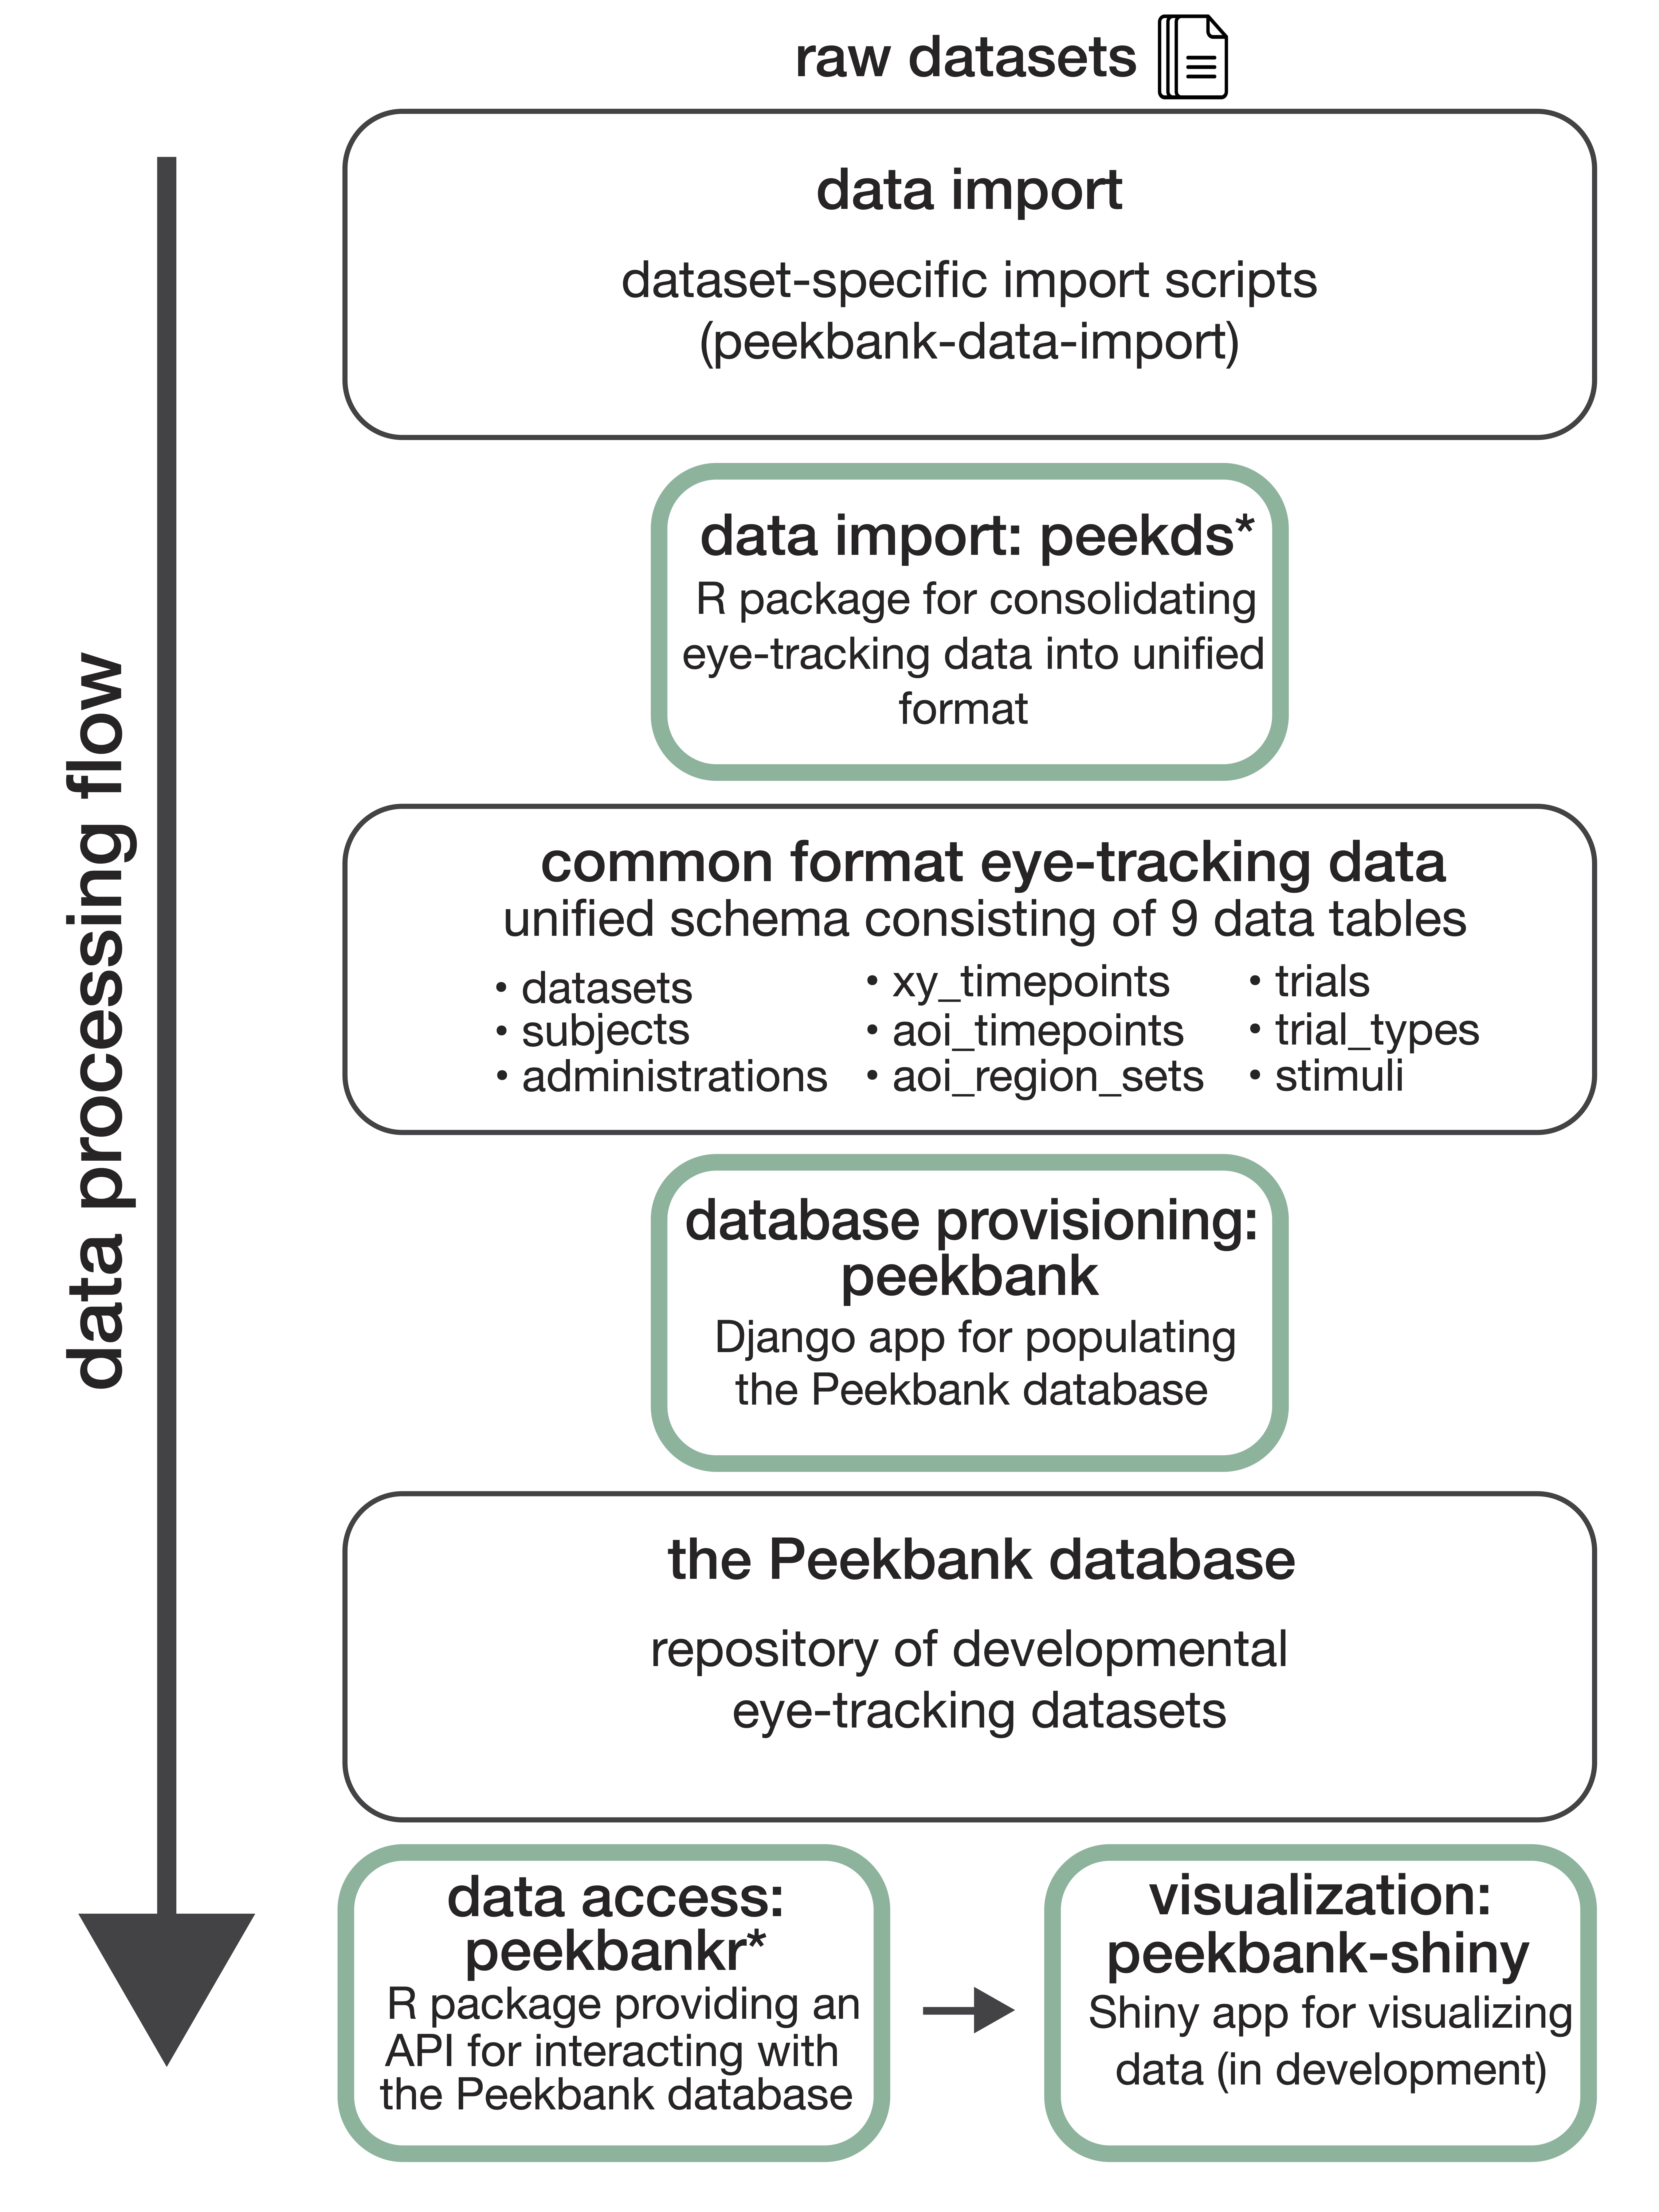
\includegraphics[width=18in,height=4.5in]{/Users/martinzettersten/GitHub/peekbank-paper/brm/figures/peekbankflowchartv6} 

}

\caption{Overview of the Peekbank data ecosystem. Peekbank tools are highlighted in green. * indicates R packages introduced in this work.}\label{fig:fig-framework-overview}
\end{figure}

\hypertarget{database-schema}{%
\subsection{Database Schema}\label{database-schema}}

The Peekbank database contains two major types of data: (1) metadata regarding experiments, participants, and trials, and (2) time course looking data, detailing where a child is looking on the screen at a given point in time (Fig. \ref{fig:fig-schema}).

\begin{figure}

{\centering 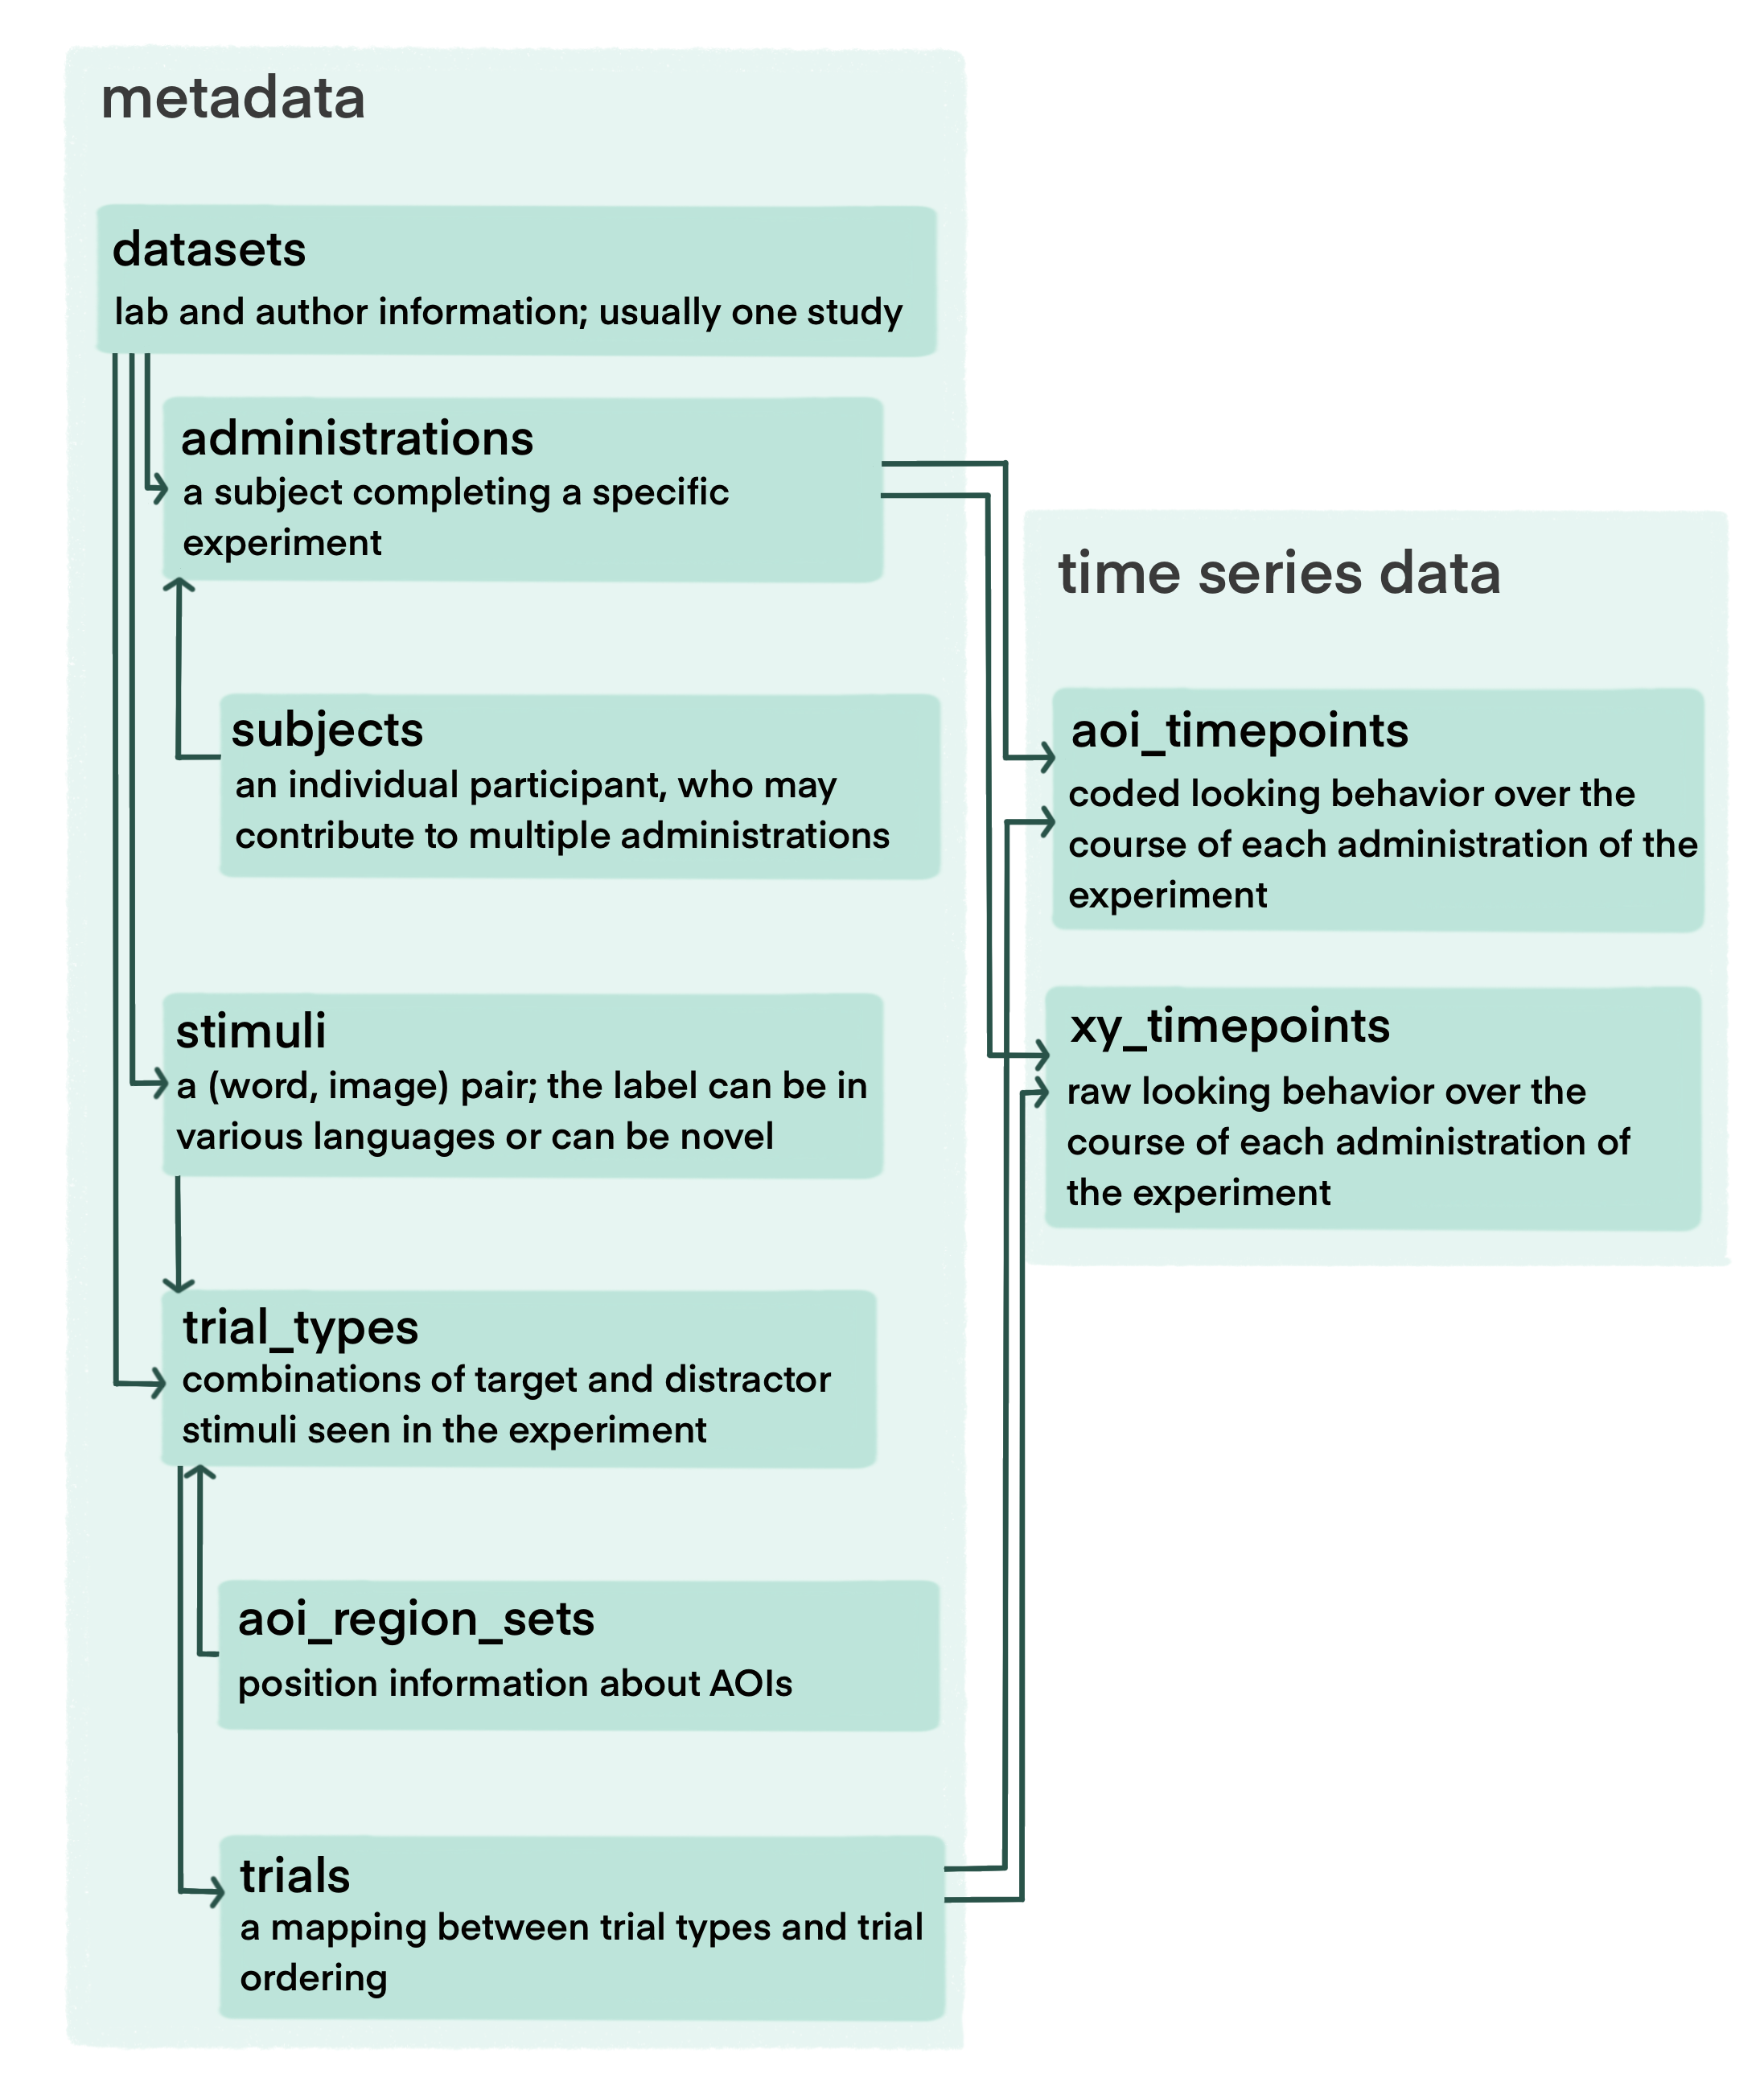
\includegraphics[width=7.31in,height=4.5in]{/Users/martinzettersten/GitHub/peekbank-paper/brm/figures/schema_3} 

}

\caption{The Peekbank schema. Each darker rectangle represents a table in the relational database.}\label{fig:fig-schema}
\end{figure}

\hypertarget{metadata}{%
\subsubsection{Metadata}\label{metadata}}

Metadata can be separated into four parts: (1) participant-level information (e.g., demographics), (2) experiment-level information (e.g., the type of eye tracker used to collect the data), (3) session information (e.g.~a participant's age for a specific experimental session), and (4) trial information (e.g., which images or videos were presented onscreen, and paired with which audio).

\hypertarget{participant-information}{%
\paragraph{Participant Information}\label{participant-information}}

All information about individual participants in Peekbank is completely de-identified under United States law, containing none of the key identifiers listed under the ``Safe Harbor'' standard for data de-identification.
All participant-level linkages are made using anonymous participant identifiers.

Invariant information about individuals who participate in one or more studies (e.g, a participant's first language) is recorded in the \texttt{subjects} table, while the \texttt{administrations} table contains information about each individual session in a given study (see Session Information, below).
This division allows Peekbank to gracefully handle longitudinal designs: a single participant can complete multiple sessions and thus be associated with multiple administrations.

Participant-level data includes all participants who have experiment data.
In general, we include as many participants as possible in the database and leave it to end-users to apply the appropriate exclusion criteria for their analysis.

\hypertarget{experiment-information}{%
\paragraph{Experiment Information}\label{experiment-information}}

The \texttt{datasets} table includes information about the lab conducting the study and the relevant publications to cite regarding the data.
In most cases, a dataset corresponds to a single study.

Information about the experimental design is split across the \texttt{trial\_types} and \texttt{stimuli} tables.
The \texttt{trial\_types} table encodes information about each trial \textit{in the design of the experiment},\footnote{We note that the term \textit{trial} is ambiguous and could be used to refer to both a particular combination of stimuli seen by many participants and a participant seeing that particular combination at a particular point in the experiment. We track the former in the \texttt{trial\_types} table and the latter in the \texttt{trials} table.} including the target stimulus and location (left vs.~right), the distractor stimulus and location, and the point of disambiguation for that trial.
If a dataset used automatic eye-tracking rather than manual coding, each trial type is additionally linked to a set of area of interest (x, y) coordinates, encoded in the \texttt{aoi\_region\_sets} table.
The \texttt{trial\_types} table links trial types to the \texttt{aoi\_region\_sets} table and the \texttt{trials} table.
Each trial\_type record links to two records in the \texttt{stimuli} table, identified by the \texttt{distractor\_id} and the \texttt{target\_id} fields.

Each record in the \texttt{stimuli} table is a (word, image) pair.
In most experiments, there is a one-to-one mapping between images and labels (e.g., each time an image of a dog appears it is referred to as \emph{dog}).
For studies in which there are multiple potential labels per image (e.g., \emph{dog} and \emph{chien} are both used to refer to an image of a dog), images can have multiple rows in the \texttt{stimuli} table with unique labels.
This structure is useful for studies on synonymy or using multiple languages.
It is also possible for an image to be associated with a row with no label, if the image appears solely as a distractor (and thus its label is ambiguous).
For studies in which the same label refers to multiple images (e.g., the word \emph{dog} refers to an image of a dalmatian and a poodle), the same label can have multiple rows in the \texttt{stimuli} table with unique images.

\hypertarget{session-information}{%
\paragraph{Session Information}\label{session-information}}

The \texttt{administrations} table includes information about the participant or experiment that may change between sessions of the same study, even for the same participant.
This includes the age of the participant, the coding method (eye-tracking vs.~hand-coding), and the properties of the monitor that was used.
For participant age, we include the fields \texttt{lab\_age} and \texttt{lab\_age\_units} to record how the original lab encoded age, as well as an additional field, \texttt{age}, to encode age in a standardized format across datasets, using months as the common unit of measurement.

\hypertarget{trial-information}{%
\paragraph{Trial Information}\label{trial-information}}

The \texttt{trials} table includes information about a specific participant completing a specific instance of a trial type.
This table links each record in the time course looking data (described below) to the trial type and specifies the order of the trials seen by a specific participant.

\hypertarget{time-course-data}{%
\subsubsection{Time course data}\label{time-course-data}}

Raw looking data is a series of looks to areas of interest (AOIs), such as looks to the left or right of the screen, or to (x, y) coordinates on the experiment screen, linked to points in time.
For data generated by eye-trackers, we typically have (x, y) coordinates at each time point, which we encode in the \texttt{xy\_timepoints} table.
These looks are also recoded into AOIs according to the AOI coordinates in the \texttt{aoi\_region\_sets} table using the \texttt{add\_aois()} function in \texttt{peekds}, and encoded in the \texttt{aoi\_timepoints} table.
For hand-coded data, we typically have a series of AOIs (i.e., looks to the left vs.~right of the screen), but lack information about exact gaze positions on-screen; in these cases the AOIs are recoded into the categories in the Peekbank schema (target, distractor, other, and missing) and encoded in the \texttt{aoi\_timepoints} table; however, these datasets do not have any corresponding data in the \texttt{xy\_timepoints} table.

Typically, timepoints in the \texttt{xy\_timepoints} table and \texttt{aoi\_timepoints} table need to be regularized to center each trial's time around the point of disambiguation -- such that 0 is the time of target word onset in the trial (i.e., the beginning of \emph{dog} in \emph{Can you find the dog?}).
We re-centered timing information to the onset of the target label to facilitate comparison of target label processing across all datasets.\footnote{While information preceding the onset of the target label in some datasets such as co-articulation cues (Mahr, McMillan, Saffran, Ellis Weismer, \& Edwards, 2015) or adjectives (Fernald, Marchman, \& Weisleder, 2013) can in principle disambiguate the target referent, we use a standardized point of disambiguation based on the onset of the label for the target referent. Onset times for other potentially disambiguating information (such as adjectives) can typically be recovered from the raw data provided on OSF.}
If time values run throughout the experiment rather than resetting to zero at the beginning of each trial, \texttt{rezero\_times()} is used to reset the time at each trial.
After this, each trial's times are centered around the point of disambiguation using \texttt{normalize\_times()}.
When these steps are complete, the time course is ready for resampling.

To facilitate time course analysis and visualization across datasets, time course data must be resampled to a uniform sampling rate (i.e., such that every trial in every dataset has observations at the same time points).
All data in the database is resampled to 40 Hz (observations every 25 ms), which represents a compromise between retaining fine-grained timing information from datasets with dense sampling rates (maximum sampling rate among current datasets: 500 Hz) while minimizing the possibility of introducing artifacts via resampling for datasets with lower sampling rates (minimum sampling rate for current datasets: 30 Hz).
Further, 25 ms is a mathematically convenient interval for ensuring consistent resampling; we found that using 33.333 ms (30 Hz) as our interval simply introduced a large number of technical complexities.
The resampling operation is accomplished using the \texttt{resample\_times()} function.
During the resampling process, we interpolate using constant interpolation, selecting for each interpolated timepoint the looking location for the earlier-observed time point in the original data for both \texttt{aoi\_timepoints} and \texttt{xy\_timepoints} data.
Compared to linear interpolation (see e.g., Wass, Smith, \& Johnson, 2013) -- which fills segments of missing or unobserved time points by interpolating between the observed locations of timepoints at the beginning and end of the interpolated segment --, constant interpolation has the advantage that it is more conservative, in the sense that it does not introduce new look locations beyond those measured in the original data.
One possible application of our new dataset is investigating the consequences of other interpolation functions for data analysis.

\hypertarget{processing-validation-and-ingestion}{%
\subsection{Processing, Validation, and Ingestion}\label{processing-validation-and-ingestion}}

Although Peekbank provides a common data format, the crux issue of populating the database is the conversion of existing datasets to this format.
Each dataset is imported via a custom import script, which documents the process of conversion.
Often various decisions must be made in this import process (for example, how to characterize a particular trial type within the options available in the Peekbank schema); these scripts provide a reproducible record of this decision-making process. Our data import repository (available on GitHub at \url{https://github.com/langcog/peekbank-data-import}) contains all of these scripts, links to internal documentation on data import, and a set of generic import templates for different formats.

Many of the specific operations involved in importing a dataset can be abstracted across datasets.
The \texttt{peekds} package offers a library of these functions.
Once the data have been extracted in a tabular form, the package also offers a validation function that checks whether all tables have the required fields and data types expected by the database.
In an effort to double check the data quality and to make sure that no errors are made in the importing script, we also typically perform a visual check of the import process, creating a time course plot to replicate the results in the paper that first presented each dataset
Once this plot has been created and checked for consistency and all tables pass our validation functions, the processed dataset is ready for reprocessing into the database using the \texttt{peekbank} library.
This library applies additional data checks, and adds the data to the MySQL database using the Django web framework.

To date, the import process has been carried out by the Peekbank team using data offered by other research teams.
There is no technical obstacle to data contributors also providing an import script to facilitate contribution, though in practice creating these scripts requires familiarity with both R scripting and the specific Peekbank schema; writing a first import script can be somewhat time-consuming.
To support future data contributions, import script templates and examples are available for both hand-coded datasets and automatic eye-tracking datasets for research teams to adapt to their data.
These import templates walk researchers through each step of data processing using example datasets from Peekbank and include explanations of key decision points, examples of how to use various helper functions available in \texttt{peekds}, and further details about the database schema.

\hypertarget{current-data-sources}{%
\subsection{Current Data Sources}\label{current-data-sources}}

\begin{table}

\caption{\label{tab:dataset-table}Overview of the datasets in the current database.}
\centering
\resizebox{\linewidth}{!}{
\begin{tabular}[t]{llrrlll}
\toprule
Study Citation & Dataset name & N & Mean age (mos.) & Age range (mos.) & Method & Language\\
\midrule
Adams et al., 2018 & adams\_marchman\_2018 & 69 & 17.1 & 13–20 & manual coding & English\\
Byers-Heinlein et al., 2017 & byers-heinlein\_2017 & 48 & 20.1 & 19–21 & eye-tracking & English, French\\
Casillas et al., 2017 & casillas\_tseltal\_2015 & 23 & 31.3 & 9–48 & manual coding & Tseltal\\
Fernald et al., 2013 & fmw\_2013 & 80 & 20.0 & 17–26 & manual coding & English\\
Frank et al., 2016 & frank\_tablet\_2016 & 69 & 35.5 & 12–60 & eye-tracking & English\\
Garrison et al., 2020 & garrison\_bergelson\_2020 & 35 & 14.5 & 12–18 & eye-tracking & English\\
Hurtado et al., 2007 & xsectional\_2007 & 49 & 23.8 & 15–37 & manual coding & Spanish\\
Hurtado et al., 2008 & hurtado\_2008 & 76 & 21.0 & 17–27 & manual coding & Spanish\\
Mahr et al., 2015 & mahr\_coartic & 29 & 20.8 & 18–24 & eye-tracking & English\\
Perry et al., 2017 & perry\_cowpig & 45 & 20.5 & 19–22 & manual coding & English\\
Pomper \& Saffran, 2016 & pomper\_saffran\_2016 & 60 & 44.3 & 41–47 & manual coding & English\\
Pomper \& Saffran, 2019 & pomper\_salientme & 44 & 40.1 & 38–43 & manual coding & English\\
Potter \& Lew-Williams, unpub. & potter\_canine & 36 & 23.8 & 21–27 & manual coding & English\\
Potter et al., 2019 & potter\_remix & 44 & 22.6 & 18–29 & manual coding & Spanish, English\\
Ronfard et al., 2021 & ronfard\_2021 & 40 & 20.0 & 18–24 & manual coding & English\\
Swingley \& Aslin, 2002 & swingley\_aslin\_2002 & 50 & 15.1 & 14–16 & manual coding & English\\
Weisleder \& Fernald, 2013 & weisleder\_stl & 29 & 21.6 & 18–27 & manual coding & Spanish\\
Yurovsky \& Frank, 2017 & attword\_processed & 288 & 25.5 & 13–59 & eye-tracking & English\\
Yurovsky et al., 2013 & reflook\_socword & 435 & 33.6 & 12–70 & eye-tracking & English\\
Yurovsky et al., unpub. & reflook\_v4 & 45 & 34.2 & 11–60 & eye-tracking & English\\
\bottomrule
\end{tabular}}
\end{table}

The database currently includes 20 looking-while-listening datasets comprising \emph{N}=1594 total participants (Table 1).
The current data represents a convenience sample of datasets that were (a) datasets collected by or available to Peekbank team members, (b) made available to Peekbank after informal inquiry or (c) datasets that were openly available.
Most datasets (14 out of 20 total) consist of data from monolingual native English speakers.
They span a wide age spectrum with participants ranging from 9 to 70 months of age, and are balanced in terms of gender (47.30\% female; 50.40\% male; 2.30\% unreported).
The datasets vary across a number of design-related dimensions, and include studies using manually coded video recordings and automated eye-tracking methods (e.g., Tobii, EyeLink) to measure gaze behavior.
All studies tested familiar items, but the database also includes 5 datasets that tested novel pseudo-words in addition to familiar words.
Users interested in a subset of the data (e.g., only trials testing familiar words) can filter out unwanted trials using columns available in the schema (e.g., using the column \texttt{stimulus\_novelty} in the \texttt{stimuli} table).

\hypertarget{versioning-and-reproducibility}{%
\subsection{Versioning and Reproducibility}\label{versioning-and-reproducibility}}

The content of Peekbank will change as we add additional datasets and revise previous ones.
To facilitate reproducibility of analyses, we use a versioning system by which successive releases are assigned a name reflecting the year and version, e.g., \texttt{2022.1}.
By default, users will interact with the most recent version of the database available, though the \texttt{peekbankr} API allows researchers to run analyses against any previous version of the database.
For users with intensive use-cases, each version of the database may be downloaded as a compressed .sql file and installed on a local MySQL server.

Peekbank allows for fully reproducible analyses using our source data, but the goal is not to reproduce precisely the analyses -- or even the datasets -- in the publications whose data we archive. Because of our emphasis on a standardized data importing and formatting pipeline, there may be minor discrepancies in the time course data that we archive compared with those reported in original publications. Further, we archive all of the data that are provided to us -- including participants that might have been excluded in the original studies, if these data are available -- rather than attempting to reproduce specific exclusion criteria. We hope that Peekbank can be used as a basis for comparing different exclusion and filtering criteria -- as such, an inclusive policy regarding importing all available data helps us provide a broad base of data for investigating these decisions.

\hypertarget{interfacing-with-peekbank}{%
\section{Interfacing with Peekbank}\label{interfacing-with-peekbank}}

\hypertarget{peekbankr}{%
\subsection{Peekbankr}\label{peekbankr}}

The \texttt{peekbankr} API offers a way for users to access data from the database and flexibly analyze it in \texttt{R}. The majority of API calls simply allow users to download tables (or subsets of tables) from the database. In particular, the package offers the following functions:

\begin{itemize}
\tightlist
\item
  \texttt{connect\_to\_peekbank()} opens a connection with the Peekbank database to allow tables to be downloaded with the following functions
\item
  \texttt{get\_datasets()} gives each dataset name and its citation information
\item
  \texttt{get\_subjects()} gives information about persistent participant identifiers (e.g., native languages, sex)
\item
  \texttt{get\_administrations()} gives information about specific experimental administrations (e.g., participant age, monitor size, gaze coding method)
\item
  \texttt{get\_stimuli()} gives information about word--image pairings that appeared in experiments\\
\item
  \texttt{get\_trial\_types()} gives information about pairings of stimuli that appeared in the experiment (e.g., point of disambiguation, target and distractor stimuli, condition, language)
\item
  \texttt{get\_trials()} gives the trial orderings for each administration, linking trial types to the trial IDs used in time course data
\item
  \texttt{get\_aoi\_region\_sets()} gives coordinate regions for each area of interest (AOI) linked to trial type IDs
\item
  \texttt{get\_xy\_timepoints()} gives time course data for each participant's looking behavior in each trial, as (x, y) coordinates on the experiment monitor
\item
  \texttt{get\_aoi\_timepoints()} gives time course data for each participant's looking behavior in each trial, coded into areas of interest
\end{itemize}

Once users have downloaded tables, they can be merged using \texttt{join} commands via their linked IDs. A set of standard merges are shown below in the ``Peekbank in Action'' section; these allow the common use-case of examining time course data and metadata jointly.

Because of the size of the XY and AOI data tables, downloading data across multiple studies can be time-consuming. Many of the most common analyses of the Peekbank data require downloading the \texttt{aoi\_timepoints} table, thus we have put substantial work into optimizing transfer times. In particular, \texttt{connect\_to\_peekbank} offers a data compression option, and \texttt{get\_aoi\_timepoints} by default downloads time courses via a compressed (run-length encoded) representation, which is then uncompressed on the client side. More information about these options (including how to modify them) can be found in the package documentation.

\hypertarget{shiny-app}{%
\subsection{Shiny App}\label{shiny-app}}

One goal of the Peekbank project is to allow a wide range of users to easily explore and learn from the database.
We therefore have created an interactive web application -- \texttt{peekbank-shiny} -- that allows users to quickly and easily create informative visualizations of individual datasets and aggregated data (\url{https://peekbank-shiny.com/}).
\texttt{peekbank-shiny} is built using Shiny, a software package for creating web apps for data exploration with R, as well as the \texttt{peekbankr} package.
All code for the Shiny app is publicly available (\url{https://github.com/langcog/peekbank-shiny}).
The Shiny app allows users to create commonly used visualizations of looking-while-listening data, based on data from the Peekbank database.
Specifically, users can visualize:

\begin{enumerate}
\def\labelenumi{\arabic{enumi}.}
\tightlist
\item
  the \emph{time course of looking data} in a profile plot depicting infant target looking across trial time
\item
  \emph{overall accuracy}, defined as the proportion target looking within a specified analysis window
\item
  \emph{reaction times} in response to a target label, defined as how quickly participants shift fixation to the target image on trials in which they were fixating on the distractor image at onset of the target label
\item
  an \emph{onset-contingent plot}, which shows the time course of participant looking as a function of their look location at the onset of the target label
\end{enumerate}

Users are given various customization options for each of these visualizations, e.g., choosing which datasets to include in the plots, controlling the age range of participants, splitting the visualizations by age bins, and controlling the analysis window for time course analyses.
Plots are then updated in real time to reflect users' customization choices.
A screenshot of the app is shown in Figure \ref{fig:shiny}.
The Shiny app thus allows users to quickly inspect basic properties of Peekbanks datasets and create reproducible visualizations without incurring any of the technical overhead required to access the database through R.

\begin{figure}

{\centering 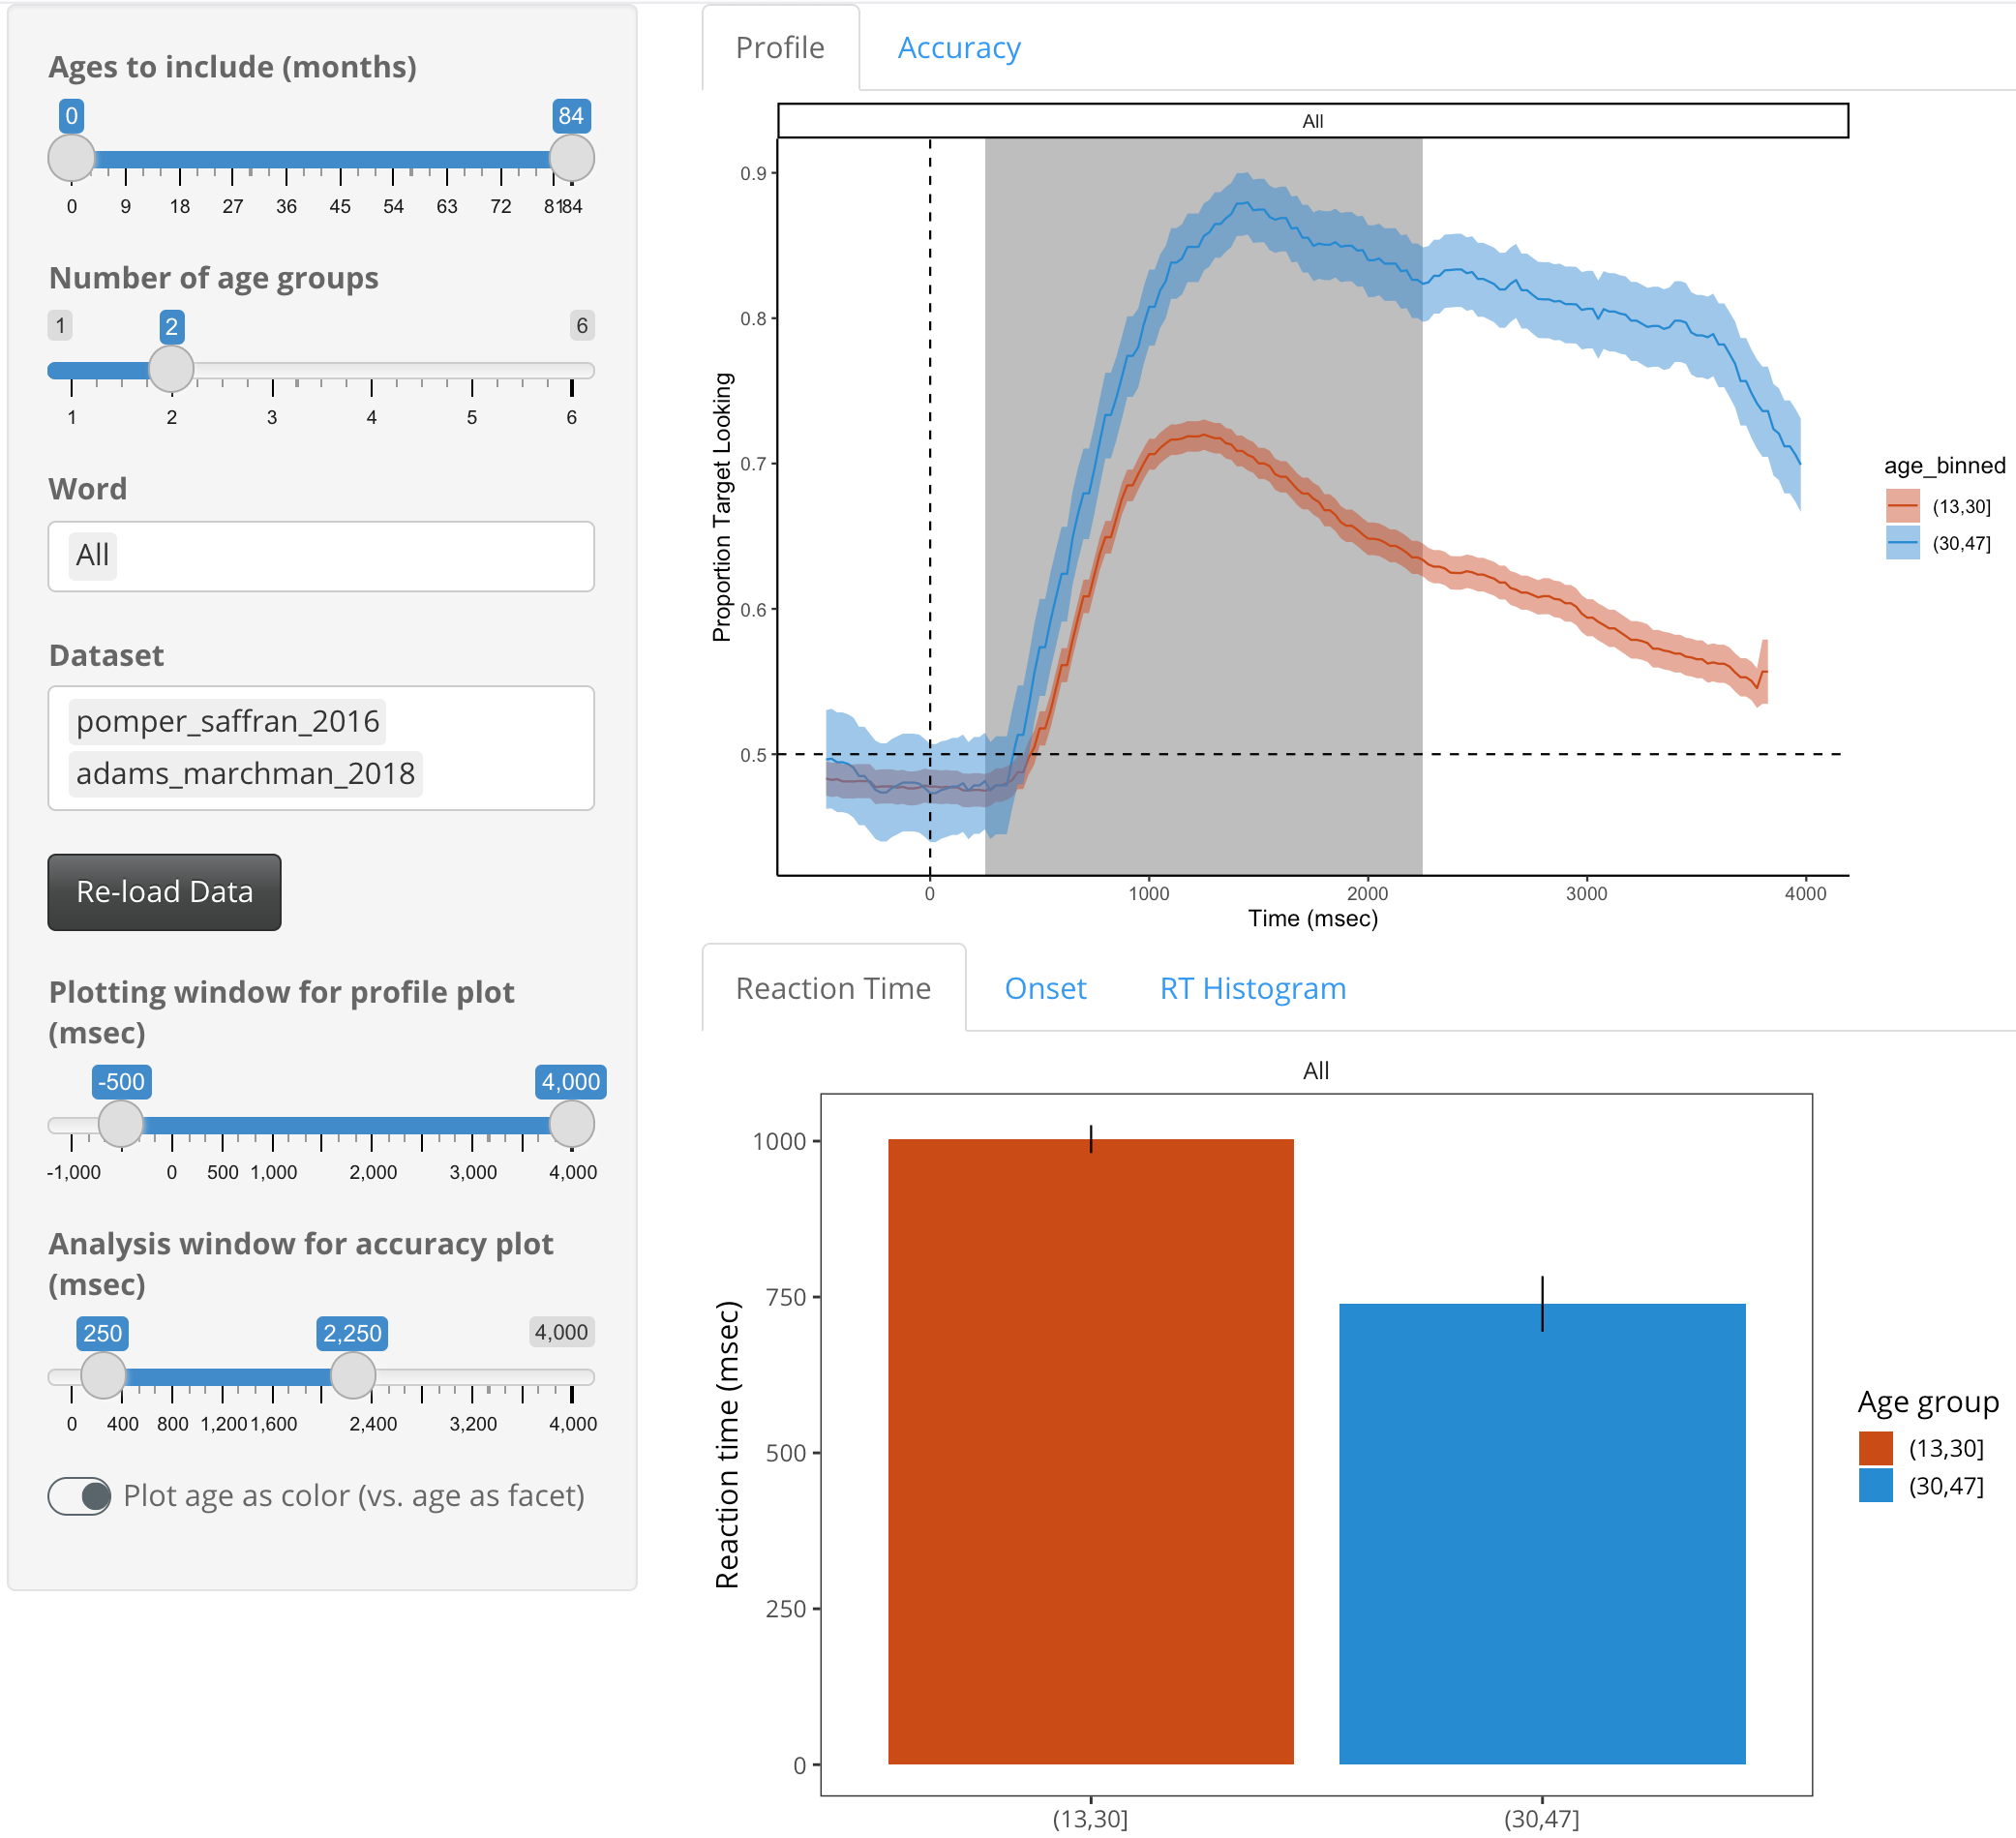
\includegraphics[width=6.94in,height=6in]{/Users/martinzettersten/GitHub/peekbank-paper/brm/figures/shiny-full-window} 

}

\caption{Screenshot of the Peekbank Shiny app, which shows a variety of standard analysis plots as a function of user-selected datasets, words, age ranges, and analysis windows. Shown here are mean reaction time and proportion target looking over time by age group for two selected datasets.}\label{fig:shiny}
\end{figure}

\hypertarget{osf-site}{%
\subsection{OSF site}\label{osf-site}}

In addition to the Peekbank database proper, all data is openly available on the Peekbank OSF webpage (\url{https://osf.io/pr6wu/}).
The OSF site also includes the original raw data (both time series data and metadata, such as trial lists and participant logs) that was obtained for each study and subsequently processed into the standardized Peekbank format.
Where available, the OSF page also includes additional information about the stimuli used in each dataset, including in some instances the original stimulus sets (e.g., image and audio files).

\hypertarget{peekbank-in-action}{%
\section{Peekbank in Action}\label{peekbank-in-action}}

In the following section, we provide examples of how users can access and analyze the data in Peekbank.
First, we provide an overview of some general properties of the datasets in the database.
We then demonstrate two potential use-cases for Peekbank data.
In each case, we provide sample code to demonstrate the ease of doing simple analyses using the database.
Our first example shows how we can investigate the findings of a classic study.
This type of investigation can be a very useful exercise for teaching students about best practices for data analysis (e.g., Hardwicke et al., 2018) and also provides an easy way to explore looking-while-listening time course data in a standardized format.
Our second example shows an exploration of developmental changes in the recognition of particular words.
Besides its theoretical interest (which we will explore more fully in subsequent work), this type of analysis could in principle be used for optimizing the stimuli for new experiments, especially as the Peekbank dataset grows and gains coverage over a greater number of items.
All analyses are conducted using R {[}Version 4.1.1; R Core Team (2021){]}\footnote{We, furthermore, used the R-packages \emph{dplyr} {[}Version 1.0.7; Wickham, François, Henry, and Müller (2021){]}, \emph{forcats} {[}Version 0.5.1; Wickham (2021a){]}, \emph{ggplot2} {[}Version 3.3.5; Wickham (2016){]}, \emph{ggthemes} {[}Version 4.2.4; Arnold (2021){]}, \emph{here} {[}Version 1.0.1; Müller (2020){]}, \emph{papaja} {[}Version 0.1.0.9997; Aust and Barth (2020){]}, \emph{peekbankr} {[}Version 0.1.1.9002; Braginsky, MacDonald, and Frank (2021){]}, \emph{purrr} {[}Version 0.3.4; Henry and Wickham (2020){]}, \emph{readr} {[}Version 2.0.1; Wickham and Hester (2021){]}, \emph{stringr} {[}Version 1.4.0; Wickham (2019){]}, \emph{tibble} {[}Version 3.1.4; Müller and Wickham (2021){]}, \emph{tidyr} {[}Version 1.1.3; Wickham (2021b){]}, \emph{tidyverse} {[}Version 1.3.1; Wickham et al. (2019){]}, \emph{tinylabels} (Barth, 2021), \emph{viridis} {[}Version 0.6.1; Garnier et al. (2021a); Garnier et al. (2021b){]}, \emph{viridisLite} {[}Version 0.4.0; Garnier et al. (2021b){]}, and \emph{xtable} {[}Version 1.8.4; Dahl, Scott, Roosen, Magnusson, and Swinton (2019){]}.}

\hypertarget{general-descriptives}{%
\subsection{General Descriptives}\label{general-descriptives}}

\begin{table}[H]
\centering
\begingroup\fontsize{9pt}{10pt}\selectfont
\begin{tabular}{lrrl}
  \hline
Study Citation & Unique Items & Prop. Target & 95\% CI \\ 
  \hline
Adams et al., 2018 & 8 & 0.65 & [0.63, 0.67] \\ 
  Byers-Heinlein et al., 2017 & 6 & 0.55 & [0.52, 0.58] \\ 
  Casillas et al., 2017 & 30 & 0.59 & [0.54, 0.63] \\ 
  Fernald et al., 2013 & 12 & 0.65 & [0.63, 0.67] \\ 
  Frank et al., 2016 & 24 & 0.64 & [0.6, 0.68] \\ 
  Garrison et al., 2020 & 87 & 0.60 & [0.56, 0.64] \\ 
  Hurtado et al., 2007 & 8 & 0.59 & [0.55, 0.63] \\ 
  Hurtado et al., 2008 & 12 & 0.61 & [0.59, 0.63] \\ 
  Mahr et al., 2015 & 10 & 0.71 & [0.68, 0.74] \\ 
  Perry et al., 2017 & 12 & 0.61 & [0.58, 0.63] \\ 
  Pomper \& Saffran, 2016 & 40 & 0.77 & [0.75, 0.8] \\ 
  Pomper \& Saffran, 2019 & 16 & 0.74 & [0.72, 0.75] \\ 
  Potter \& Lew-Williams, unpub. & 16 & 0.65 & [0.61, 0.68] \\ 
  Potter et al., 2019 & 8 & 0.63 & [0.58, 0.67] \\ 
  Ronfard et al., 2021 & 8 & 0.69 & [0.65, 0.73] \\ 
  Swingley \& Aslin, 2002 & 22 & 0.57 & [0.55, 0.59] \\ 
  Weisleder \& Fernald, 2013 & 12 & 0.63 & [0.6, 0.66] \\ 
  Yurovsky \& Frank, 2017 & 6 & 0.63 & [0.62, 0.65] \\ 
  Yurovsky et al., 2013 & 6 & 0.61 & [0.6, 0.63] \\ 
  Yurovsky et al., unpub. & 10 & 0.61 & [0.57, 0.65] \\ 
   \hline
\end{tabular}
\endgroup
\caption{Average proportion target looking in each dataset.} 
\end{table}

One of the values of the uniform data format we use in Peekbank is the ease of providing cross-dataset descriptions that can give an overview of some of the general patterns found in our data.
A first broad question is about the degree of accuracy in word recognition found across studies.
In general, participants demonstrated robust, above-chance word recognition in each dataset (chance=0.5).
Table 2 shows the average proportion of target looking within a standard critical window of 367-2000ms after the onset of the label for each dataset (Swingley \& Aslin, 2002).
Proportion target looking was generally higher for familiar words (\emph{M} = 0.66, 95\% CI = {[}0.65, 0.67{]}, \emph{n} = 1543) than for novel words learned during the experiment (\emph{M} = 0.59, 95\% CI = {[}0.58, 0.61{]}, \emph{n} = 822).

\begin{figure}
\centering
\includegraphics{peekbank-brm_files/figure-latex/items-1.pdf}
\caption{\label{fig:items}Item-level variability in proportion target looking within each dataset (chance=0.5). Time is centered on the onset of the target label (vertical line). Colored lines represent specific target labels. Black lines represent smoothed average fits based on a general additive model using cubic splines.}
\end{figure}

A second question of interest is about the variability across items (i.e., target labels) within specific studies. Some studies use a smaller set of items (e.g., 8 nouns, Adams et al., 2018) while others use dozens of different items (e.g., Garrison, Baudet, Breitfeld, Aberman, \& Bergelson, 2020). Figure \ref{fig:items} gives an overview of the variability in proportion looking to the target item for individual words in each dataset. Although all datasets show a gradual rise in average proportion target looking over chance performance, the number of unique target labels and their associated accuracy vary widely across datasets.

\hypertarget{investigating-prior-findings-swingley2002}{%
\subsection{Investigating prior findings: Swingley and Aslin (2002)}\label{investigating-prior-findings-swingley2002}}

Swingley and Aslin (2002) investigated the specificity of 14-16-month-olds' word representations using the looking-while-listening paradigm, asking whether recognition would be slower and less accurate for mispronunciations, e.g.~\emph{opal} (mispronunciation) instead of \emph{apple} (correct pronunciation).\footnote{The original paper investigated both close (e.g., \emph{opple}, /apl/) and distant (e.g., \emph{opal}, /opl/) mispronunciations. For simplicity, here we combine both mispronunciation conditions since the close vs.~distant mispronunciation manipulation showed no effect in the original paper.} In this short vignette, we show how easily the data in Peekbank can be used to visualize this result. Our goal here is not to provide a precise analytical reproduction of the analyses reported in the original paper, but rather to demonstrate the use of the Peekbank framework to analyze datasets of this type. In particular, because Peekbank uses a uniform data import standard, it is likely that there will be minor numerical discrepancies between analyses on Peekbank data and analyses that use another processing pipeline.

\singlespacing

\begin{Shaded}
\begin{Highlighting}[]
\FunctionTok{library}\NormalTok{(peekbankr)}
\NormalTok{aoi\_timepoints }\OtherTok{\textless{}{-}} \FunctionTok{get\_aoi\_timepoints}\NormalTok{(}\AttributeTok{dataset\_name =} \StringTok{"swingley\_aslin\_2002"}\NormalTok{)}
\NormalTok{administrations }\OtherTok{\textless{}{-}} \FunctionTok{get\_administrations}\NormalTok{(}\AttributeTok{dataset\_name =} \StringTok{"swingley\_aslin\_2002"}\NormalTok{)}
\NormalTok{trial\_types }\OtherTok{\textless{}{-}} \FunctionTok{get\_trial\_types}\NormalTok{(}\AttributeTok{dataset\_name =} \StringTok{"swingley\_aslin\_2002"}\NormalTok{)}
\NormalTok{trials }\OtherTok{\textless{}{-}} \FunctionTok{get\_trials}\NormalTok{(}\AttributeTok{dataset\_name =} \StringTok{"swingley\_aslin\_2002"}\NormalTok{)}
\end{Highlighting}
\end{Shaded}

\doublespacing

We begin by retrieving the relevant tables from the database, \texttt{aoi\_timepoints}, \texttt{administrations}, \texttt{trial\_types}, and \texttt{trials}. As discussed above, each of these can be downloaded using a simple API call through \texttt{peekbankr}, which returns dataframes that include ID fields. These ID fields allow for easy joining of the data into a single dataframe containing all of the information necessary for the analysis.

\singlespacing

\begin{Shaded}
\begin{Highlighting}[]
\NormalTok{swingley\_data }\OtherTok{\textless{}{-}}\NormalTok{ aoi\_timepoints }\SpecialCharTok{|}\ErrorTok{\textgreater{}}
  \FunctionTok{left\_join}\NormalTok{(administrations) }\SpecialCharTok{|}\ErrorTok{\textgreater{}}
  \FunctionTok{left\_join}\NormalTok{(trials) }\SpecialCharTok{|}\ErrorTok{\textgreater{}}
  \FunctionTok{left\_join}\NormalTok{(trial\_types) }\SpecialCharTok{|}\ErrorTok{\textgreater{}}
  \FunctionTok{filter}\NormalTok{(condition }\SpecialCharTok{!=} \StringTok{"filler"}\NormalTok{) }\SpecialCharTok{|}\ErrorTok{\textgreater{}}
  \FunctionTok{mutate}\NormalTok{(}\AttributeTok{condition =} \FunctionTok{if\_else}\NormalTok{(condition }\SpecialCharTok{==} \StringTok{"cp"}\NormalTok{, }\StringTok{"Correct"}\NormalTok{, }\StringTok{"Mispronounced"}\NormalTok{))}
\end{Highlighting}
\end{Shaded}

\doublespacing

As the code above shows, once the data are joined, condition information for each timepoint is present and so we can easily filter out filler trials and set up the conditions for further analysis.

\singlespacing

\begin{Shaded}
\begin{Highlighting}[]
\NormalTok{accuracies }\OtherTok{\textless{}{-}}\NormalTok{ swingley\_data  }\SpecialCharTok{|}\ErrorTok{\textgreater{}}
  \FunctionTok{group\_by}\NormalTok{(condition, t\_norm, administration\_id) }\SpecialCharTok{|}\ErrorTok{\textgreater{}} 
  \FunctionTok{summarize}\NormalTok{(}\AttributeTok{correct =} \FunctionTok{sum}\NormalTok{(aoi }\SpecialCharTok{==} \StringTok{"target"}\NormalTok{) }\SpecialCharTok{/} 
              \FunctionTok{sum}\NormalTok{(aoi }\SpecialCharTok{\%in\%} \FunctionTok{c}\NormalTok{(}\StringTok{"target"}\NormalTok{,}\StringTok{"distractor"}\NormalTok{))) }\SpecialCharTok{|}\ErrorTok{\textgreater{}}
  \FunctionTok{group\_by}\NormalTok{(condition, t\_norm) }\SpecialCharTok{|}\ErrorTok{\textgreater{}} 
  \FunctionTok{summarize}\NormalTok{(}\AttributeTok{mean\_correct =} \FunctionTok{mean}\NormalTok{(correct),}
            \AttributeTok{ci =} \FloatTok{1.96} \SpecialCharTok{*} \FunctionTok{sd}\NormalTok{(correct) }\SpecialCharTok{/} \FunctionTok{sqrt}\NormalTok{(}\FunctionTok{n}\NormalTok{()))}
\end{Highlighting}
\end{Shaded}

\doublespacing

The final step in our analysis is to create a summary dataframe using \texttt{dplyr} commands. We first group the data by timestep, participant, and condition and compute the proportion looking at the correct image. We then summarize again, averaging across participants, computing both means and 95\% confidence intervals (via the approximation of 1.96 times the standard error of the mean). The resulting dataframe can be used for visualization of the time course of looking.

\begin{figure}
\centering
\includegraphics{peekbank-brm_files/figure-latex/swingley-1.pdf}
\caption{\label{fig:swingley}Proportion looking at the correct referent by time from the point of disambiguation (the onset of the target noun) in Swingley \& Aslin (2002). Colors show the two pronunciation conditions; points give means and ranges show 95\% confidence intervals. The dotted line shows the point of disambiguation and the dashed line shows chance performance.}
\end{figure}

Figure \ref{fig:swingley} shows the average time course of looking for the two conditions, as produced by the code above. Looks after the correctly pronounced noun appeared both faster (deviating from chance earlier) and more accurate (showing a higher asymptote). Overall, this example demonstrates the ability to produce this visualization in just a few lines of code.

\hypertarget{item-analyses}{%
\subsection{Item analyses}\label{item-analyses}}

A second use-case for Peekbank is to examine item-level variation in word recognition. Individual datasets rarely have enough statistical power to show reliable developmental differences within items. To illustrate the power of aggregating data across multiple datasets, we select the four words with the most data available across studies and ages (apple, book, dog, and frog) and show average recognition trajectories.

Our first step is to collect and join the data from the relevant tables including timepoint data, trial and stimulus data, and administration data (for participant ages). We join these into a single dataframe for easy manipulation; this dataframe is a common starting point for analyses of item-level data.

\begin{Shaded}
\begin{Highlighting}[]
\NormalTok{all\_aoi\_timepoints }\OtherTok{\textless{}{-}} \FunctionTok{get\_aoi\_timepoints}\NormalTok{()}
\NormalTok{all\_stimuli }\OtherTok{\textless{}{-}} \FunctionTok{get\_stimuli}\NormalTok{()}
\NormalTok{all\_administrations }\OtherTok{\textless{}{-}} \FunctionTok{get\_administrations}\NormalTok{()}
\NormalTok{all\_trial\_types }\OtherTok{\textless{}{-}} \FunctionTok{get\_trial\_types}\NormalTok{() }
\NormalTok{all\_trials }\OtherTok{\textless{}{-}} \FunctionTok{get\_trials}\NormalTok{()  }

\NormalTok{aoi\_data\_joined }\OtherTok{\textless{}{-}}\NormalTok{ all\_aoi\_timepoints }\SpecialCharTok{|}\ErrorTok{\textgreater{}}
  \FunctionTok{right\_join}\NormalTok{(all\_administrations) }\SpecialCharTok{|}\ErrorTok{\textgreater{}}
  \FunctionTok{right\_join}\NormalTok{(all\_trials) }\SpecialCharTok{|}\ErrorTok{\textgreater{}}
  \FunctionTok{right\_join}\NormalTok{(all\_trial\_types) }\SpecialCharTok{|}\ErrorTok{\textgreater{}}
  \FunctionTok{mutate}\NormalTok{(}\AttributeTok{stimulus\_id =}\NormalTok{ target\_id) }\SpecialCharTok{|}\ErrorTok{\textgreater{}}
  \FunctionTok{right\_join}\NormalTok{(all\_stimuli) }\SpecialCharTok{|}\ErrorTok{\textgreater{}}
  \FunctionTok{select}\NormalTok{(administration\_id, english\_stimulus\_label, age, t\_norm, aoi)}
\end{Highlighting}
\end{Shaded}

Next we select a set of four target words (chosen based on having more than 100 children contributing data for each word across several one-year age groups).
We create age groups, aggregate, and compute timepoint-by-timepoint confidence intervals using the \(z\) approximation.

\begin{Shaded}
\begin{Highlighting}[]
\NormalTok{target\_words }\OtherTok{\textless{}{-}} \FunctionTok{c}\NormalTok{(}\StringTok{"book"}\NormalTok{,}\StringTok{"dog"}\NormalTok{,}\StringTok{"frog"}\NormalTok{,}\StringTok{"apple"}\NormalTok{)}

\NormalTok{target\_word\_data }\OtherTok{\textless{}{-}}\NormalTok{ aoi\_data\_joined }\SpecialCharTok{|}\ErrorTok{\textgreater{}}
  \FunctionTok{filter}\NormalTok{(english\_stimulus\_label }\SpecialCharTok{\%in\%}\NormalTok{ target\_words) }\SpecialCharTok{|}\ErrorTok{\textgreater{}}
  \FunctionTok{mutate}\NormalTok{(}\AttributeTok{age\_group =} \FunctionTok{cut}\NormalTok{(age, }\AttributeTok{breaks =} \FunctionTok{seq}\NormalTok{(}\DecValTok{12}\NormalTok{,}\DecValTok{48}\NormalTok{,}\DecValTok{12}\NormalTok{))) }\SpecialCharTok{|}\ErrorTok{\textgreater{}}
  \FunctionTok{filter}\NormalTok{(}\SpecialCharTok{!}\FunctionTok{is.na}\NormalTok{(age\_group)) }\SpecialCharTok{|}\ErrorTok{\textgreater{}}
  \FunctionTok{group\_by}\NormalTok{(t\_norm, administration\_id, age\_group, english\_stimulus\_label) }\SpecialCharTok{|}\ErrorTok{\textgreater{}} 
  \FunctionTok{summarise}\NormalTok{(}\AttributeTok{correct =} \FunctionTok{sum}\NormalTok{(aoi }\SpecialCharTok{==} \StringTok{"target"}\NormalTok{) }\SpecialCharTok{/} 
              \FunctionTok{sum}\NormalTok{(aoi }\SpecialCharTok{\%in\%} \FunctionTok{c}\NormalTok{(}\StringTok{"target"}\NormalTok{,}\StringTok{"distractor"}\NormalTok{))) }\SpecialCharTok{|}\ErrorTok{\textgreater{}}
  \FunctionTok{group\_by}\NormalTok{(t\_norm, age\_group, english\_stimulus\_label) }\SpecialCharTok{|}\ErrorTok{\textgreater{}} 
  \FunctionTok{summarise}\NormalTok{(}\AttributeTok{ci =} \FloatTok{1.96} \SpecialCharTok{*} \FunctionTok{sd}\NormalTok{(correct, }\AttributeTok{na.rm=}\ConstantTok{TRUE}\NormalTok{) }\SpecialCharTok{/} \FunctionTok{sqrt}\NormalTok{(}\FunctionTok{length}\NormalTok{(correct)), }
            \AttributeTok{correct =} \FunctionTok{mean}\NormalTok{(correct, }\AttributeTok{na.rm=}\ConstantTok{TRUE}\NormalTok{), }
            \AttributeTok{n =} \FunctionTok{n}\NormalTok{()) }
\end{Highlighting}
\end{Shaded}

Finally, we plot the data as time courses split by age. Our plotting code is shown below (with styling commands removed for clarity). Figure \ref{fig:target-word-plot} shows the resulting plot, with time courses for each of three (rather coarse) age bins.
Although some baseline effects are visible across items, we still see clear and consistent increases in looking to the target, with the increase appearing earlier and in many cases asymptoting at a higher level for older children.

\begin{Shaded}
\begin{Highlighting}[]
\FunctionTok{ggplot}\NormalTok{(target\_word\_data, }
       \FunctionTok{aes}\NormalTok{(}\AttributeTok{x =}\NormalTok{ t\_norm, }\AttributeTok{y =}\NormalTok{ correct, }\AttributeTok{col =}\NormalTok{ age\_group)) }\SpecialCharTok{+} 
  \FunctionTok{geom\_line}\NormalTok{() }\SpecialCharTok{+} 
  \FunctionTok{geom\_linerange}\NormalTok{(}\FunctionTok{aes}\NormalTok{(}\AttributeTok{ymin =}\NormalTok{ correct }\SpecialCharTok{{-}}\NormalTok{ ci, }\AttributeTok{ymax =}\NormalTok{ correct }\SpecialCharTok{+}\NormalTok{ ci), }
                 \AttributeTok{alpha =}\NormalTok{ .}\DecValTok{2}\NormalTok{) }\SpecialCharTok{+} 
  \FunctionTok{facet\_wrap}\NormalTok{(}\SpecialCharTok{\textasciitilde{}}\NormalTok{english\_stimulus\_label)}
\end{Highlighting}
\end{Shaded}

\begin{figure}
\centering
\includegraphics{peekbank-brm_files/figure-latex/target-word-plot-1.pdf}
\caption{\label{fig:target-word-plot}Time course plot for four well-represented target items in the Peekbank dataset, split by three age groups. Each line represents children's average looking to the target image after the onset of the target label (dashed vertical line). Error bars represent 95\% CIs.}
\end{figure}

This simple averaging approach is a proof-of-concept to demonstrate some of the potential of the Peekbank dataset.
An eye-movement trajectory on an individual trial reflects myriad factors, including the age and ability of the child, the target and distractor stimuli on that trial, the position of the trial within the experiment, and the general parameters of the experiment (for example, stimulus timing, eye-tracker type and calibration, etc.).
Although we often neglect these statistically in the analysis of individual experiments -- for example, averaging across items and trial orders -- they may lead to imprecision when we average across multiple studies in Peekbank.
For example, studies with older children may use more difficult items or faster trial timing, leading to the impression that children's abilities overall increase more slowly than they do in fact.
Even in our example in Figure \ref{fig:target-word-plot}, we see hints of this confounding -- for example, the low baseline looks to \emph{apple} may be an artifact of an attractive distractor being paired with this item in one or two studies.
In future work, we hope to introduce model-based analytic methods that use mixed effects regression to factor out study-level and individual-level variance in order to recover developmental effects more appropriately (see e.g., Zettersten et al., 2021 for a prototype of such an analysis).

\hypertarget{discussion}{%
\section{Discussion}\label{discussion}}

Theoretical progress in understanding child development requires rich datasets, but collecting child data is expensive, difficult, and time-intensive.
Recent years have seen a growing effort to build open source tools and pool research efforts to meet the challenge of building a cumulative developmental science (Bergmann et al., 2018; Frank, Braginsky, Yurovsky, \& Marchman, 2017; Sanchez et al., 2019; The ManyBabies Consortium, 2020).
The Peekbank project expands on these efforts by building an infrastructure for aggregating eye-tracking data across studies, with a specific focus on the looking-while-listening paradigm.
This paper presents an overview of the structure of the database, shows how users can access the database, and demonstrates how it can be used both to investigate prior experiments and to synthesize data across studies.

The current database has a number of limitations, particularly in the number and diversity of datasets it contains.
With 20 datasets currently available in the database, idiosyncrasies of particular designs and condition manipulations still have a substantial influence on the results of particular analyses, as discussed above in our item analysis example.
Expanding the set of distinct datasets will allow us to increase the number of datasets that contain specific items, leading to more robust generalizations across the many sources of variation that are confounded within studies (e.g., item set, participant age range, and specific experimental parameters).
A critical next step will be the development of analytic models that take this structure into account in making generalizations across datasets.

A second limitation stems from the fact that the database represents a convenience sample of data readily available to the Peekbank team, which leads the database to be relatively homogeneous in a number of key respects.
First, the datasets primarily come from labs that share similar theoretical perspectives and implement the looking-while-listening method in similar ways.
The current database is also limited by the relatively homogeneous background of its participants, both with respect to language (almost entirely monolingual native English speakers) and cultural background (Henrich, Heine, \& Norenzayan, 2010; Muthukrishna et al., 2020).
Increasing the diversity of lab sources, participant backgrounds, and languages will expand the scope of the generalizations we can form about child word recognition, while also providing new opportunities for describing cross-lab, cross-cultural, and cross-linguistic variation.

Towards the goal of expanding our database, we invite researchers to contribute their data.
On the Peekbank website, we provide technical documentation for potential contributors.
Although we anticipate being involved in most new data imports, as discussed above, our import process is transparently documented and the repository contains examples for most commonly-used eye-trackers.
Contributing data to an open repository also can raise questions about participant privacy.
Potential contributors should consult with their local institutional review boards for guidance on any challenges, but we do not foresee obstacles because of the de-identified nature of the data.
Under United States regulation, all data contributed to Peekbank are considered de-identified and hence not considered ``human subjects data''; hence, institutional review boards should not regulate this contribution process.
Under the European Union's Generalized Data Protection Regulation (GDPR), labs may need to take special care to provide a separate set of participant identifiers that can never be re-linked to their own internal records.

While the current database is focused on studies of word recognition, the tools and infrastructure developed in the project can in principle be used to accommodate any eye-tracking paradigm, opening up new avenues for insights into cognitive development.
Gaze behavior has been at the core of many key advances in our understanding of infant cognition (Aslin, 2007; Baillargeon, Spelke, \& Wasserman, 1985; Bergelson \& Swingley, 2012; Fantz, 1963; Liu, Ullman, Tenenbaum, \& Spelke, 2017; Quinn, Eimas, \& Rosenkrantz, 1993).
Aggregating large datasets of infant looking behavior in a single, openly-accessible format promises to bring a fuller picture of infant cognitive development into view.

\newpage

\hypertarget{references}{%
\section{References}\label{references}}

\begingroup
\setlength{\parindent}{-0.5in}
\setlength{\leftskip}{0.5in}

\hypertarget{refs}{}
\begin{CSLReferences}{1}{0}
\leavevmode\hypertarget{ref-Adams2018}{}%
Adams, K. A., Marchman, V. A., Loi, E. C., Ashland, M. D., Fernald, A., \& Feldman, H. M. (2018). {Caregiver talk and medical risk as predictors of language outcomes in full term and preterm toddlers}. \emph{Child Development}, \emph{89}(5), 1674--1690.

\leavevmode\hypertarget{ref-R-ggthemes}{}%
Arnold, J. B. (2021). \emph{Ggthemes: Extra themes, scales and geoms for 'ggplot2'}. Retrieved from \url{https://CRAN.R-project.org/package=ggthemes}

\leavevmode\hypertarget{ref-Aslin2007}{}%
Aslin, R. N. (2007). {What's in a look?} \emph{Developmental Science}, \emph{10}(1), 48--53.

\leavevmode\hypertarget{ref-R-papaja}{}%
Aust, F., \& Barth, M. (2020). \emph{{papaja}: {Create} {APA} manuscripts with {R Markdown}}. Retrieved from \url{https://github.com/crsh/papaja}

\leavevmode\hypertarget{ref-Baillargeon1985}{}%
Baillargeon, R., Spelke, E. S., \& Wasserman, S. (1985). {Object permanence in five-month-old infants}. \emph{Cognition}, \emph{20}(3), 191--208. \url{https://doi.org/10.1016/0010-0277(85)90008-3}

\leavevmode\hypertarget{ref-Balota2007}{}%
Balota, D. A., Yap, M. J., Cortese, M. J., Hutchison, K. A., Kessler, B., Loftis, B., \ldots{} Treiman, R. (2007). {The English Lexicon project}. \emph{Behavior Research Methods}, \emph{39}(3), 445--459. \url{https://doi.org/10.3758/BF03193014}

\leavevmode\hypertarget{ref-R-tinylabels}{}%
Barth, M. (2021). \emph{{tinylabels}: Lightweight variable labels}. Retrieved from \url{https://github.com/mariusbarth/tinylabels}

\leavevmode\hypertarget{ref-bergelson2020}{}%
Bergelson, E. (2020). The comprehension boost in early word learning: Older infants are better learners. \emph{Child Development Perspectives}, \emph{14}(3), 142--149.

\leavevmode\hypertarget{ref-bergelson2012}{}%
Bergelson, E., \& Swingley, D. (2012). {At 6-9 months, human infants know the meanings of many common nouns.} \emph{Proceedings of the National Academy of Sciences}, \emph{109}(9), 3253--3258.

\leavevmode\hypertarget{ref-bergelson2013}{}%
Bergelson, E., \& Swingley, D. (2013). {{T}he acquisition of abstract words by young infants}. \emph{Cognition}, \emph{127}(3), 391--397.

\leavevmode\hypertarget{ref-bergmann2018}{}%
Bergmann, C., Tsuji, S., Piccinini, P. E., Lewis, M. L., Braginsky, M., Frank, M. C., \& Cristia, A. (2018). {Promoting replicability in developmental research through meta-analyses: Insights from language acquisition research}. \emph{Child Development}, \emph{89}(6), 1996--2009.

\leavevmode\hypertarget{ref-bleses2016}{}%
Bleses, D., Makransky, G., Dale, P. S., Højen, A., \& Ari, B. A. (2016). {Early productive vocabulary predicts academic achievement 10 years later}. \emph{Applied Psycholinguistics}, \emph{37}(6), 1461--1476.

\leavevmode\hypertarget{ref-R-peekbankr}{}%
Braginsky, M., MacDonald, K., \& Frank, M. (2021). \emph{Peekbankr: Accessing the peekbank database}. Retrieved from \url{http://github.com/langcog/peekbankr}

\leavevmode\hypertarget{ref-Byers-Heinlein2021}{}%
Byers-Heinlein, K., Bergmann, C., \& Savalei, V. (2021). {Six solutions for more reliable infant research.} \emph{Infant and Child Development}. https://doi.org/\url{https://doi.org/10.1002/icd.2296}

\leavevmode\hypertarget{ref-R-xtable}{}%
Dahl, D. B., Scott, D., Roosen, C., Magnusson, A., \& Swinton, J. (2019). \emph{Xtable: Export tables to LaTeX or HTML}. Retrieved from \url{https://CRAN.R-project.org/package=xtable}

\leavevmode\hypertarget{ref-DeBolt2020}{}%
DeBolt, M. C., Rhemtulla, M., \& Oakes, L. M. (2020). {Robust data and power in infant research: A case study of the effect of number of infants and number of trials in visual preference procedures}. \emph{Infancy}, \emph{25}(4), 393--419. \url{https://doi.org/10.1111/infa.12337}

\leavevmode\hypertarget{ref-Fantz1963}{}%
Fantz, R. L. (1963). {Pattern vision in newborn infants}. \emph{Science}, \emph{140}(3564), 296--297.

\leavevmode\hypertarget{ref-Fernald2013}{}%
Fernald, A., Marchman, V. A., \& Weisleder, A. (2013). {SES differences in language processing skill and vocabulary are evident at 18 months}. \emph{Developmental Science}, \emph{16}(2), 234--248. \url{https://doi.org/10.1111/desc.12019}

\leavevmode\hypertarget{ref-fernald1998}{}%
Fernald, A., Pinto, J. P., Swingley, D., Weinberg, A., \& McRoberts, G. W. (1998). Rapid gains in speed of verbal processing by infants in the 2nd year. \emph{Psychological Science}, \emph{9}(3), 228--231.

\leavevmode\hypertarget{ref-fernald2008}{}%
Fernald, A., Zangl, R., Portillo, A. L., \& Marchman, V. A. (2008). {Looking while listening: Using eye movements to monitor spoken language comprehension by infants and young children}. In I. A. Sekerina, E. M. Fernandez, \& H. Clahsen (Eds.), \emph{Developmental psycholinguistics: On-line methods in children's language processing} (pp. 97--135). Amsterdam: John Benjamins.

\leavevmode\hypertarget{ref-Frank2017a}{}%
Frank, M. C., Bergelson, E., Bergmann, C., Cristia, A., Floccia, C., Gervain, J., \ldots{} Yurovsky, D. (2017). {A collaborative approach to infant research: Promoting reproducibility, best practices, and theory-building}. \emph{Infancy}, \emph{22}(4), 421--435. \url{https://doi.org/10.1111/infa.12182}

\leavevmode\hypertarget{ref-frank2017}{}%
Frank, M. C., Braginsky, M., Yurovsky, D., \& Marchman, V. A. (2017). {Wordbank: An open repository for developmental vocabulary data}. \emph{Journal of Child Language}, \emph{44}(3), 677--694.

\leavevmode\hypertarget{ref-frank2021}{}%
Frank, M. C., Braginsky, M., Yurovsky, D., \& Marchman, V. A. (2021). \emph{{Variability and Consistency in Early Language Learning: The Wordbank Project}}. Cambridge, MA: MIT Press.

\leavevmode\hypertarget{ref-R-viridis}{}%
Garnier, Simon, Ross, Noam, Rudis, Robert, \ldots{} Cédric. (2021a). \emph{{viridis} - colorblind-friendly color maps for r}. \url{https://doi.org/10.5281/zenodo.4679424}

\leavevmode\hypertarget{ref-R-viridisLite}{}%
Garnier, Simon, Ross, Noam, Rudis, Robert, \ldots{} Cédric. (2021b). \emph{{viridis} - colorblind-friendly color maps for r}. \url{https://doi.org/10.5281/zenodo.4679424}

\leavevmode\hypertarget{ref-Garrison2020}{}%
Garrison, H., Baudet, G., Breitfeld, E., Aberman, A., \& Bergelson, E. (2020). {Familiarity plays a small role in noun comprehension at 12--18 months}. \emph{Infancy}, \emph{25}(4), 458--477.

\leavevmode\hypertarget{ref-gautheron_2021}{}%
Gautheron, L., Rochat, N., \& Cristia, A. (2021). Managing, storing, and sharing long-form recordings and their annotations. \emph{PsyArXiv}. Retrieved from \url{https://doi.org/10.31234/osf.io/w8trm}

\leavevmode\hypertarget{ref-golinkoff2013}{}%
Golinkoff, R. M., Ma, W., Song, L., \& Hirsh-Pasek, K. (2013). {Twenty-five years using the intermodal preferential looking paradigm to study language acquisition: What have we learned?} \emph{Perspectives on Psychological Science}, \emph{8}(3), 316--339.

\leavevmode\hypertarget{ref-gorgolewski_brain_2016}{}%
Gorgolewski, K. J., Auer, T., Calhoun, V. D., Craddock, R. C., Das, S., Duff, E. P., \ldots{} Poldrack, R. A. (2016). The brain imaging data structure, a format for organizing and describing outputs of neuroimaging experiments. \emph{Scientific Data}, \emph{3}(1), 160044. \url{https://doi.org/10.1038/sdata.2016.44}

\leavevmode\hypertarget{ref-hardwicke2018}{}%
Hardwicke, T. E., Mathur, M. B., MacDonald, K., Nilsonne, G., Banks, G. C., Kidwell, M. C., \ldots{} Frank, M. C. (2018). {Data availability, reusability, and analytic reproducibility: Evaluating the impact of a mandatory open data policy at the journal Cognition}. \emph{Royal Society Open Science}, \emph{5}(8). \url{https://doi.org/10.1098/rsos.180448}

\leavevmode\hypertarget{ref-Henrich2010}{}%
Henrich, J., Heine, S. J., \& Norenzayan, A. (2010). {The weirdest people in the world?} \emph{Behavioral and Brain Sciences}, \emph{33}(2-3), 61--83. \url{https://doi.org/10.1017/S0140525X0999152X}

\leavevmode\hypertarget{ref-R-purrr}{}%
Henry, L., \& Wickham, H. (2020). \emph{Purrr: Functional programming tools}. Retrieved from \url{https://CRAN.R-project.org/package=purrr}

\leavevmode\hypertarget{ref-hirshpasek1987}{}%
Hirsh-Pasek, K., Cauley, K. M., Golinkoff, R. M., \& Gordon, L. (1987). {The eyes have it: Lexical and syntactic comprehension in a new paradigm}. \emph{Journal of Child Language}, \emph{14}(1), 23--45.

\leavevmode\hypertarget{ref-Hurtado2007}{}%
Hurtado, N., Marchman, V. A., \& Fernald, A. (2007). {Spoken word recognition by Latino children learning Spanish as their first language}. \emph{Journal of Child Language}, \emph{34}(2), 227--249. \url{https://doi.org/10.1017/S0305000906007896}

\leavevmode\hypertarget{ref-Hurtado2008}{}%
Hurtado, N., Marchman, V. A., \& Fernald, A. (2008). {Does input influence uptake? Links between maternal talk, processing speed and vocabulary size in Spanish-learning children}. \emph{Developmental Science}, \emph{11}(6), 31--39. \url{https://doi.org/10.1111/j.1467-7687.2008.00768.x}

\leavevmode\hypertarget{ref-Lewis2016}{}%
Lewis, M., Braginsky, M., Tsuji, S., Bergmann, C., Piccinini, P. E., Cristia, A., \& Frank, M. C. (2016). \emph{{A Quantitative Synthesis of Early Language Acquisition Using Meta-Analysis}}. \emph{PsyArXiv}. \url{https://doi.org/10.31234/osf.io/htsjm}

\leavevmode\hypertarget{ref-lewwilliams2007}{}%
Lew-Williams, C., \& Fernald, A. (2007). {Young children learning Spanish make rapid use of grammatical gender in spoken word recognition}. \emph{Psychological Science}, \emph{18}(3), 193--198.

\leavevmode\hypertarget{ref-Liu2017}{}%
Liu, S., Ullman, T. D., Tenenbaum, J. B., \& Spelke, E. S. (2017). {Ten-month-old infants infer the value of goals from the costs of actions}. \emph{Science}, \emph{358}(6366), 1038--1041. \url{https://doi.org/10.1126/science.aag2132}

\leavevmode\hypertarget{ref-macwhinney2000}{}%
MacWhinney, B. (2000). \emph{{The CHILDES Project: Tools for analyzing talk}}. Mahwah, NJ: Lawrence Erlbaum Associates.

\leavevmode\hypertarget{ref-Mahr2015}{}%
Mahr, T., McMillan, B. T. M., Saffran, J. R., Ellis Weismer, S., \& Edwards, J. (2015). {Anticipatory coarticulation facilitates word recognition in toddlers}. \emph{Cognition}, \emph{142}, 345--350. \url{https://doi.org/10.1016/j.cognition.2015.05.009}

\leavevmode\hypertarget{ref-marchman2018}{}%
Marchman, V. A., Loi, E. C., Adams, K. A., Ashland, M., Fernald, A., \& Feldman, H. M. (2018). {Speed of language comprehension at 18 months old predicts school-relevant outcomes at 54 months old in children born preterm}. \emph{Journal of Developmental {\&} Behavioral Pediatrics}, \emph{39}(3), 246--253.

\leavevmode\hypertarget{ref-muthukrishna2020}{}%
Muthukrishna, M., Bell, A. V., Henrich, J., Curtin, C. M., Gedranovich, A., McInerney, J., \& Thue, B. (2020). {Beyond Western, Educated, Industrial, Rich, and Democratic (WEIRD) psychology: Measuring and mapping scales of cultural and psychological distance}. \emph{Psychological Science}, \emph{31}(6), 678--701.

\leavevmode\hypertarget{ref-R-here}{}%
Müller, K. (2020). \emph{Here: A simpler way to find your files}. Retrieved from \url{https://CRAN.R-project.org/package=here}

\leavevmode\hypertarget{ref-R-tibble}{}%
Müller, K., \& Wickham, H. (2021). \emph{Tibble: Simple data frames}. Retrieved from \url{https://CRAN.R-project.org/package=tibble}

\leavevmode\hypertarget{ref-Nosek2021}{}%
Nosek, B. A., Hardwicke, T. E., Moshontz, H., Allard, A., Corker, K. S., Dreber, A., \ldots{} Vazire, S. (2022). {Replicability, robustness, and reproducibility in psychological science.} \emph{Annual Review of Psychology}, \emph{73}, 719--748. https://doi.org/\url{https://doi.org/10.31234/osf.io/ksfvq}

\leavevmode\hypertarget{ref-peter2019}{}%
Peter, M. S., Durrant, S., Jessop, A., Bidgood, A., Pine, J. M., \& Rowland, C. F. (2019). Does speed of processing or vocabulary size predict later language growth in toddlers? \emph{Cognitive Psychology}, \emph{115}, 101238.

\leavevmode\hypertarget{ref-PotterLewWilliamsUnpub}{}%
Potter, C., \& Lew-Williams, C. (unpublished). {Behold the canine!: How does toddlers' knowledge of typical frames and familiar words interact to influence their sentence processing?}

\leavevmode\hypertarget{ref-Quinn1993}{}%
Quinn, P. C., Eimas, P. D., \& Rosenkrantz, S. L. (1993). {Evidence for representations of perceptually similar natural categories by 3-month-old and 4-month-old infants}. \emph{Perception}, \emph{22}(4), 463--475. \url{https://doi.org/10.1068/p220463}

\leavevmode\hypertarget{ref-R-base}{}%
R Core Team. (2021). \emph{R: A language and environment for statistical computing}. Vienna, Austria: R Foundation for Statistical Computing. Retrieved from \url{https://www.R-project.org/}

\leavevmode\hypertarget{ref-Ronfard2021}{}%
Ronfard, S., Wei, R., \& Rowe, M. L. (2021). Exploring the linguistic, cognitive, and social skills underlying lexical processing efficiency as measured by the looking-while-listening paradigm. \emph{Journal of Child Language}, 1--24. \url{https://doi.org/10.1017/S0305000921000106}

\leavevmode\hypertarget{ref-Sanchez2019}{}%
Sanchez, A., Meylan, S. C., Braginsky, M., MacDonald, K. E., Yurovsky, D., \& Frank, M. C. (2019). {childes-db: A flexible and reproducible interface to the child language data exchange system}. \emph{Behavior Research Methods}, \emph{51}(4), 1928--1941. \url{https://doi.org/10.3758/s13428-018-1176-7}

\leavevmode\hypertarget{ref-Swingley2002}{}%
Swingley, D., \& Aslin, R. N. (2002). {Lexical neighborhoods and the word-form representations of 14-month-olds}. \emph{Psychological Science}, \emph{13}(5), 480--484. \url{https://doi.org/10.1111/1467-9280.00485}

\leavevmode\hypertarget{ref-manybabies2020}{}%
The ManyBabies Consortium. (2020). {Quantifying sources of variability in infancy research using the infant-directed speech preference}. \emph{Advances in Methods and Practices in Psychological Science}, \emph{3}(1), 24--52.

\leavevmode\hypertarget{ref-Tincoff1999}{}%
Tincoff, R., \& Jusczyk, P. W. (1999). {Some beginnings of word comprehension in 6-month-olds}. \emph{Psychological Science}, \emph{10}(2), 172--175. \url{https://doi.org/10.1111/1467-9280.00127}

\leavevmode\hypertarget{ref-Wass2013}{}%
Wass, S. V., Smith, T. J., \& Johnson, M. H. (2013). {Parsing eye-tracking data of variable quality to provide accurate fixation duration estimates in infants and adults.} \emph{Behavior Research Methods}, \emph{45}(1), 229--250. \url{https://doi.org/10.3758/s13428-012-0245-6}

\leavevmode\hypertarget{ref-Weisleder2013}{}%
Weisleder, A., \& Fernald, A. (2013). {Talking to children matters: Early language experience strengthens processing and builds vocabulary}. \emph{Psychological Science}, \emph{24}(11), 2143--2152. \url{https://doi.org/10.1177/0956797613488145}

\leavevmode\hypertarget{ref-R-ggplot2}{}%
Wickham, H. (2016). \emph{ggplot2: Elegant graphics for data analysis}. Springer-Verlag New York. Retrieved from \url{https://ggplot2.tidyverse.org}

\leavevmode\hypertarget{ref-R-stringr}{}%
Wickham, H. (2019). \emph{Stringr: Simple, consistent wrappers for common string operations}. Retrieved from \url{https://CRAN.R-project.org/package=stringr}

\leavevmode\hypertarget{ref-R-forcats}{}%
Wickham, H. (2021a). \emph{Forcats: Tools for working with categorical variables (factors)}. Retrieved from \url{https://CRAN.R-project.org/package=forcats}

\leavevmode\hypertarget{ref-R-tidyr}{}%
Wickham, H. (2021b). \emph{Tidyr: Tidy messy data}. Retrieved from \url{https://CRAN.R-project.org/package=tidyr}

\leavevmode\hypertarget{ref-R-tidyverse}{}%
Wickham, H., Averick, M., Bryan, J., Chang, W., McGowan, L. D., François, R., \ldots{} Yutani, H. (2019). Welcome to the {tidyverse}. \emph{Journal of Open Source Software}, \emph{4}(43), 1686. \url{https://doi.org/10.21105/joss.01686}

\leavevmode\hypertarget{ref-R-dplyr}{}%
Wickham, H., François, R., Henry, L., \& Müller, K. (2021). \emph{Dplyr: A grammar of data manipulation}. Retrieved from \url{https://CRAN.R-project.org/package=dplyr}

\leavevmode\hypertarget{ref-R-readr}{}%
Wickham, H., \& Hester, J. (2021). \emph{Readr: Read rectangular text data}. Retrieved from \url{https://CRAN.R-project.org/package=readr}

\leavevmode\hypertarget{ref-YurovskyWadeKrausUnpub}{}%
Yurovsky, D., Wade, A., Kraus, A. M., Gengoux, G. W., Hardan, A. Y., \& Frank, M. C. (unpublished). {Developmental changes in the speed of social attention in early word learning}.

\leavevmode\hypertarget{ref-zettersten2021}{}%
Zettersten, M., Bergey, C., Bhatt, N., Boyce, V., Braginsky, M., Carstensen, A., \ldots{} Frank, M. C. (2021). Peekbank: Exploring children's word recognition through an open, large-scale repository for developmental eye-tracking data. \emph{Proceedings of the 43rd Annual Conference of the Cognitive Science Society}.

\end{CSLReferences}

\endgroup


\end{document}
